\chapter{Search for \ac{MSSM} $\Pphi\to\Pgt\Pgt$}
\label{chap:httmssm}

As discussed in chapter \ref{chap:theory}, from the \ac{LHC} we have observation
of a $125~\GeV$ Higgs boson which is so far consistent with the \ac{SM}. From
chapter \ref{chap:htt-sm}, we have evidence at the $3\sigma$ level of a Higgs
boson decaying into tau leptons, which has properties consistent with the $125~\GeV$ boson
discovered in the other decay channels and consistent with the \ac{SM}.
However, as discussed in section \ref{sec:mssmhiggs}, the \ac{MSSM} is an
alternative theory to the \ac{SM} which could provide a $125~\GeV$ Higgs boson
consistent with the properties observed so far experimentally. In this theory,
we would also see two additional neutral Higgs bosons. This chapter describes
the search for the three neutral Higgs bosons of the \ac{MSSM} in the final
state of $\Pgt\Pgt$. We use the symbol $\Pphi$ to refer to any one of the three
neutral Higgs bosons, $\PH$, $\Ph$ or $\PA$. This analysis largely uses the same
techniques as the \ac{SM} $\HToTauTau$ analysis and as such this chapter focusses on the
places that the analysis is different and on the interpretation of results in
the context of the \ac{MSSM}. The results documented are the ``legacy''
\ac{MSSM} $\Pphi\to\Pgt\Pgt$ result from run 1 of the \ac{LHC} \cite{HIG-13-021}, and like for
chapter~\ref{chap:htt-sm} the information is focussed on the analysis in the
$\etau$ and $\mutau$ final states. The results shown in
section~\ref{sec:mssmresults} include the combination of all channels, which for
the \ac{MSSM} analysis includes the $\etau$, $\mutau$, $\emu$, $\tautau$ and
$\mumu$ final states. 

\section{Event Selection and Categorisation}
\label{sec:mssmEventSelection}

The inclusive selection of the candidate di-tau pair is almost exactly the same
as that used for the \ac{SM} $\HToTauTau$ analysis described in section
\ref{sec:eventSelection}, with one small exception. Due
to the fact that the $\Pgth$ $\pt$ is not directly used in the \ac{MSSM} analysis we are
able to lower the $\Pgth$ $\pt$ threshold from $30~\GeV$ to $20~\GeV$. This is useful
in the \ac{MSSM} analysis since we are interested in Higgs bosons of a
much larger mass up to $1~\TeV$ and so we must consider events up to a large
$m_{\Pgt\Pgt}$. A lower $\pt$ cut on the $\Pgth$ gives a larger overall number of events
and improves the statistics in the background templates across the $m_{\Pgt\Pgt}$ range. 
Using hadronic taus lower than $30~\GeV$ in the \ac{SM} analysis was not possible 
due to an observed data - \ac{MC} discrepancy in the $\pt$ distribution for low 
$\pt$ taus as a result of imperfect modelling of the trigger in \ac{MC}.

An alternative event categorisation is used for the \ac{MSSM} analysis. Much
like in the \ac{SM} analysis where the categorisation is used to target the different 
production modes of the Higgs, the \ac{MSSM} analysis follows a similar
strategy. Events are split into those with at least one b-tagged jet, or exactly
0 b-tagged jets, referred to as the b--tag and no b--tag category.  The
definition for a b-tagged jet is as described in section~\ref{sec:btag} and has
$\pt > 30~\GeV$ and $|\eta| < 2.4$. The b--tag
category is more sensitive to b-associated Higgs production, and the no b--tag
to gluon fusion. Figure \ref{fig:nbtag} shows the number of b-tagged jets in the
$\mutau$ channel, with the two signal contributions overlaid. It can be seen
that a large amount of the b-associated production signal still falls into the
no b--tag category, which occurs for events where the b-jets fall outside the
acceptance.

\begin{figure}[tbh]
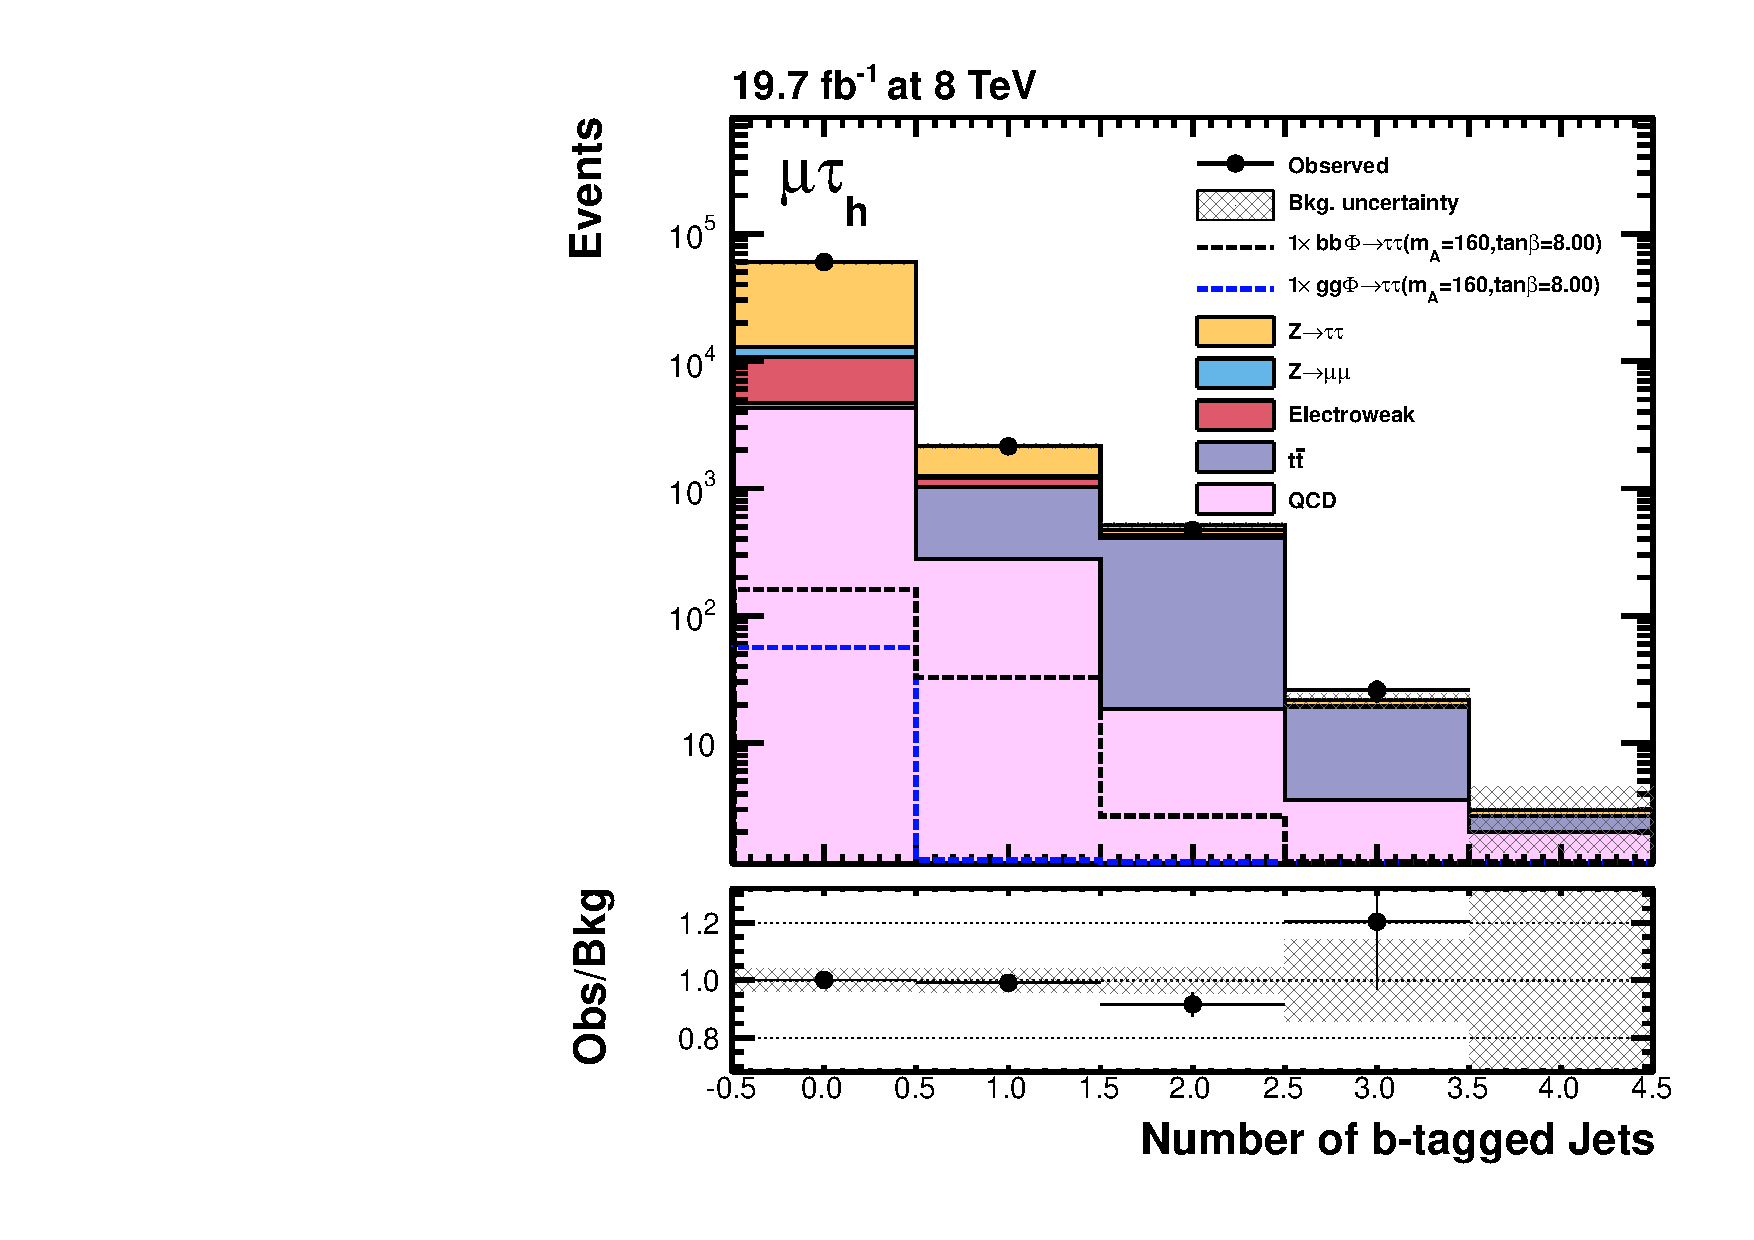
\includegraphics[width=0.6\textwidth]{plots/htt-mssm/n_bjets_inclusive_mt_2012_log.pdf}

\caption{Number of b-tagged jets in the $\mutau$ channel, as used to separate
events into b--tag and no b--tag categories. Signal contributions are shown
separately for b-associated producton and gluon fusion.}
\label{fig:nbtag}
\end{figure}

\section{Datasets and \ac{MC} samples}
\label{sec:mssmdataandMC}

The datasets and \ac{MC} samples for each of the background processes are
identical to those described in section \ref{sec:dataandMC}. The signal is
generated using \textsc{pythia}~\cite{Sjostrand:2006za} at \ac{LO}. Like the
samples described in section \ref{sec:dataandMC}, it uses \textsc{pythia}
for parton showering and hadronisation and \textsc{tauola}~\cite{TAUOLA} for tau
decays. Additional proton-proton collisions to simulate pileup events are added
as for the other samples. The signal samples are generated in a mass range from
$90~\GeV$ up to $1~\TeV$ in steps of varying size. 

\section{Background Methods and Systematics}
\label{sec:mssmBackgroundsSysts}

\subsection{Background Methods}
\label{sec:mssmBackgrounds}
The background composition is very similar to that of the \ac{SM} $\HToTauTau$
analysis and the methods used to estimate the contributions follow those
described in section \ref{sec:backgrounds}. The requirement of at least one
b-tagged jet in the b-tag category reduces background from $\ZToTauTau$
and increases the contribution of $\ttbar$. As described in section
\ref{sec:backgroundEstimation_Ztautau}, an embedding procedure is used for the
$\ZToTauTau$ estimate, in which $\PZ\to\Pgm\Pgm$ events in data are replaced
with simulated taus. It is known that a small fraction of selected data events
are $\ttbar$ events instead of $\PZ\to\Pgm\Pgm$ events, and hence it is
necessary to calculate this contamination in the b--tag category so as to avoid
double counting of $\ttbar$. The contamination is estimated by running the
embedding procedure on a $\ttbar$ \ac{MC} sample. For the $\etau$ and $\mutau$ channels, this
contamination is around $1.5\%$, and so the $\ttbar$ yield is reduced
accordingly. 

Similarly to the way cuts on $m_{jj}$ and $|\Delta\eta_{jj}|$ are relaxed to
obtain smooth shapes for the $\WJets$ background in the VBF categories, the
b-tagging working point for the jets is relaxed to the loose working point to
obtain the shape for the b--tag category. This is also done for the shape of
the $\PZ\to\ell\ell$ background. For the QCD, the same-sign data is used for
both shape and normalisation in the no--btag category, whereas for the b--tag
category the shape is taken from anti-isolated same-sign data using the relaxed
b-tagging working point.

Data to \ac{MC} corrections are the same as those used in the \ac{SM}
$\HToTauTau$ analysis as described in section~\ref{sec:datamcfactors}. An
additional correction is derived for the $\WJets$ background to account for
observed differences in the jet-tau fake-rate at high $\pt$, which in particular
affects the high mass tail of the $\WJets$. 

\subsection{Tail fitting of backgrounds}
\label{sec:tailfitting}

One large difference between the \ac{MSSM} $\Pphi\to\Pgt\Pgt$ analysis compared
with the $\HToTauTau$ analysis is the fact that we consider Higgs bosons of
masses up to $1~\TeV$. This means that we must study the $m_{\Pgt\Pgt}$
distribution up to high values of around $1.5~\TeV$. In these high mass regions, the
number of events in our backgrounds is greatly reduced, and it becomes more
difficult to obtain smooth background templates. This results in a need for a
large number of bin-by-bin uncertainties like those described in
section~\ref{sec:systematicUncertainties_shape} to cover bins with low
statistics. A better method for dealing with this is to ensure that the bins are
all populated by fitting the template in the high mass region using an analytic
function, and replacing the template with the result of that function.

The function used for the high mass fits takes the following form:

\begin{equation}
f = exp\left(\frac{-m_{\Pgt\Pgt}}{c_{0} + c_{1}\cdot m_{\Pgt\Pgt}}\right) ,
\end{equation}

where $c_{0}$ and $c_{1}$ are free parameters in the fit. The fit is made to
the \ac{MC} in the region $m_{\Pgt\Pgt} > 150~\GeV$ and then the template is
replaced by the values of the analytical function for this region. To represent
the uncertainty on this high mass fit in the final maximum-likelihood fit, shape
uncertainties are generated corresponding to the $\pm1\sigma$ shift in the fit
parameters $c_{0}$ and $c_{1}$. The values of the uncertainty $\sigma$ are the 
eigenvalues of the covariance matrix of the fit. Figure \ref{fig:tailfits} shows
an example of the fit obtained for the \WJets background in the $\mutau$
channel, showing the central fit to the template and the shape nuisances which
are added to the maximum likelihood fit.

\begin{figure}[tbh]
\subfloat[]{
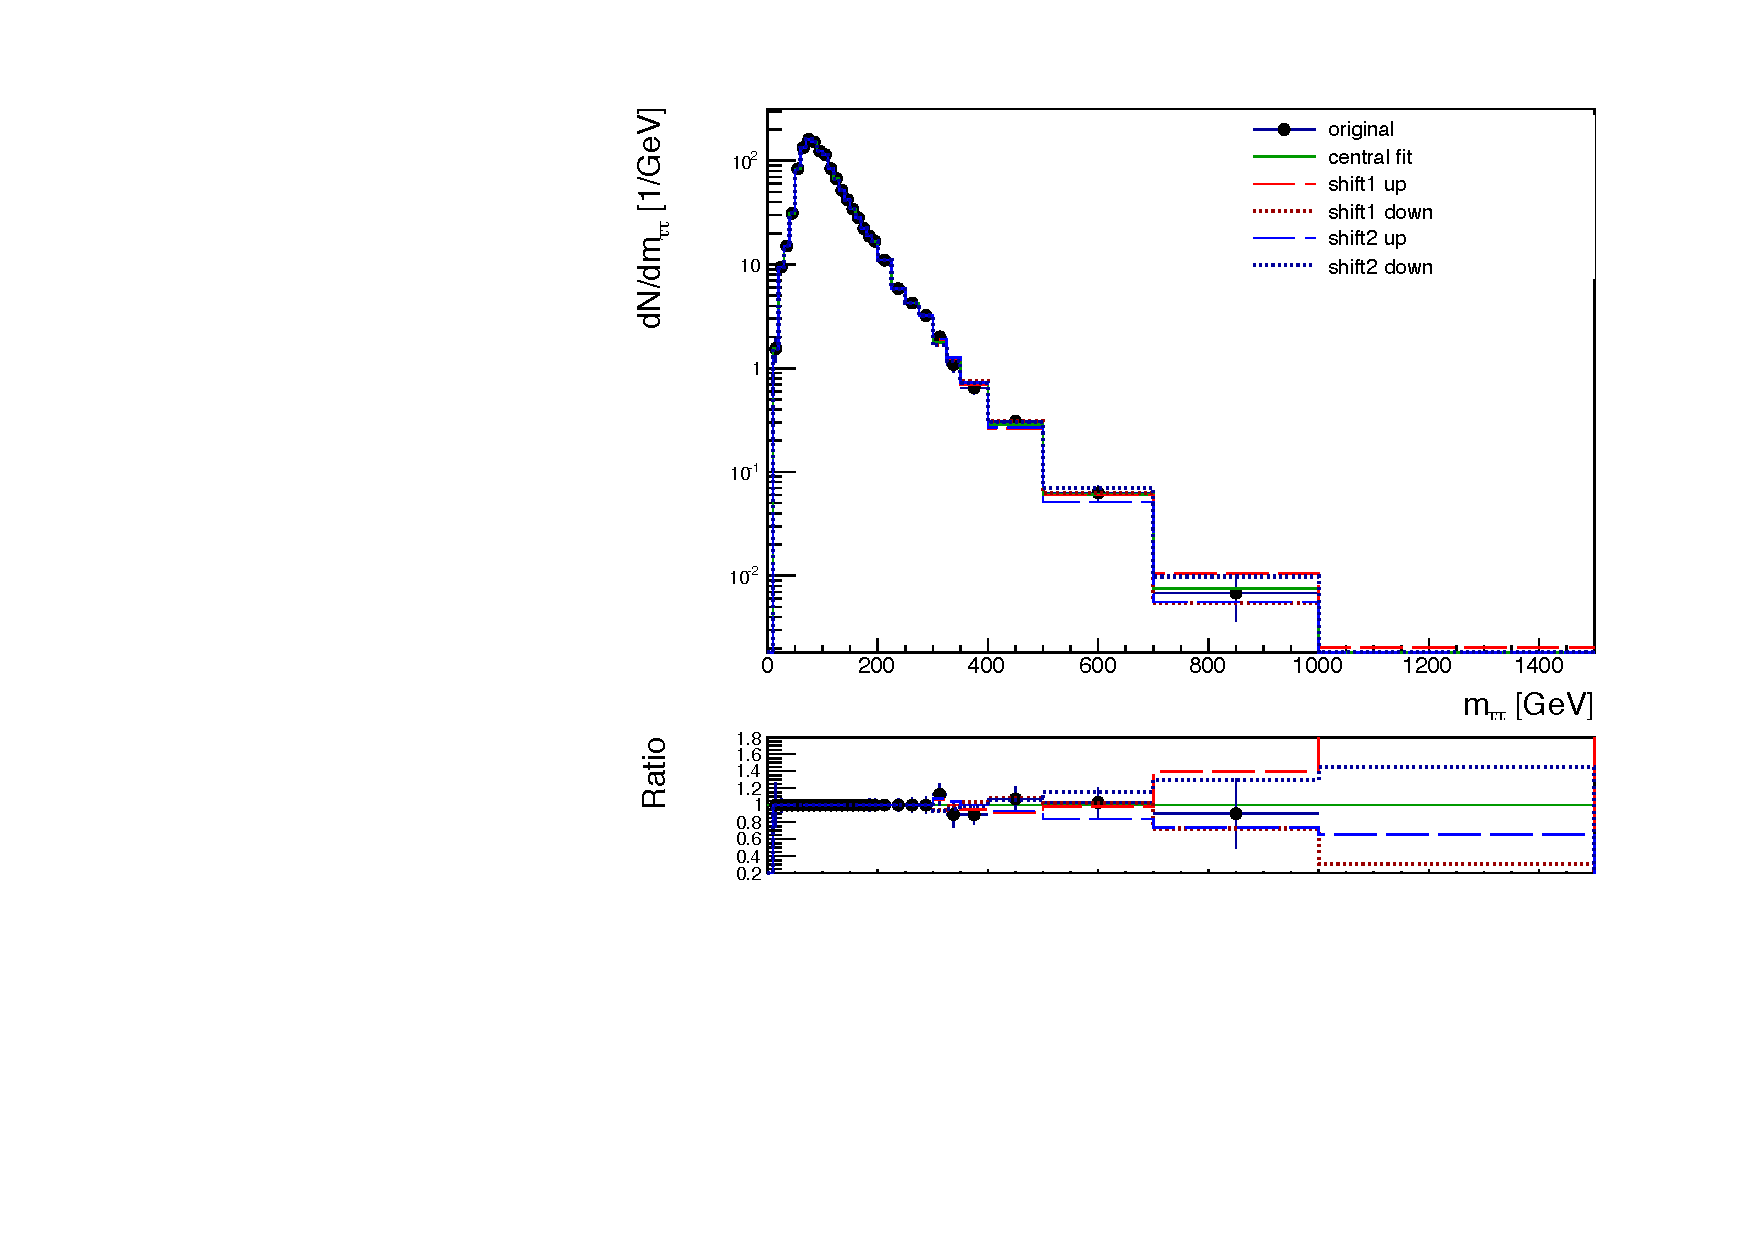
\includegraphics[width=0.5\textwidth]{plots/htt-mssm/W_fine_binning_CMS_shift1_muTau_nobtag_8TeV_Rebin.pdf}}
\subfloat[]{
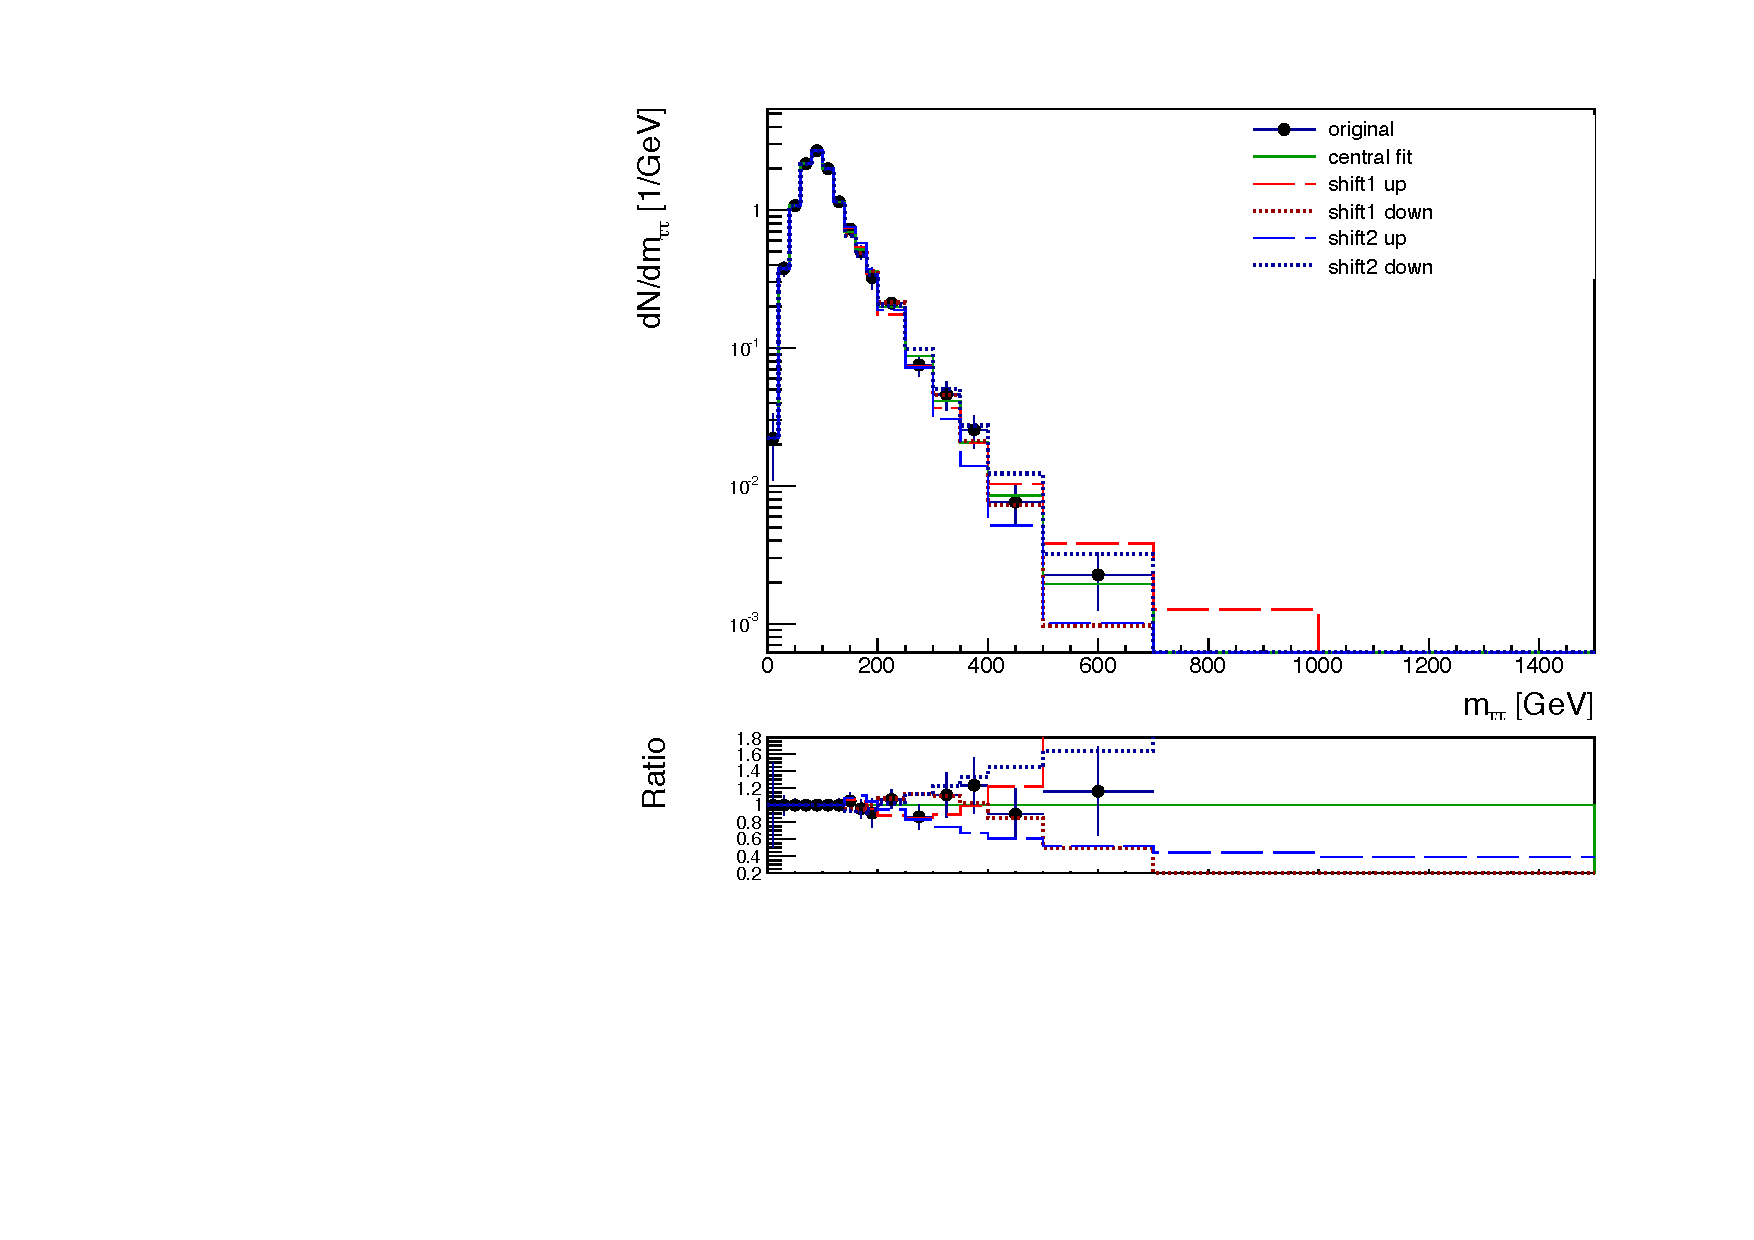
\includegraphics[width=0.5\textwidth]{plots/htt-mssm/W_fine_binning_CMS_shift1_muTau_btag_8TeV_Rebin.pdf}}
\caption{Analytic fits to the high mass tail of the $m_{\Pgt\Pgt}$ distribution,
shown here for the example of the $\WJets$ background. Fits are shown for the
no--btag (a) and b--tag (b) categories of the $\mutau$ channel in $8~\TeV$
\ac{MC}. The green line corresponds to the central fit, and the red and blue
lines indicate the systematic uncertainties added to the final
maximum-likelihood fit corresponding to the uncertainties in the two fitted
parameters.}
\label{fig:tailfits}
\end{figure}

Fits are performed for the $\WJets$, QCD and $\ttbar$ backgrounds in the $\etau$
and $\mutau$ channels, where the statistics in the templates are good enough to
produce a reliable fit. In the backgrounds in which a tail fit is not used, and
in the low mass regions of the fitted backgrounds, bin-by-bin uncertainties as
described in section~\ref{sec:systematicUncertainties_shape} are applied.

\subsection{Other Systematic Uncertainties}
%%Try to find some references for some of these things
The majority of the systematic uncertainties in the \ac{MSSM} analysis are the
same as those in the \ac{SM} analysis as described in
section~\ref{sec:systematics}, with evaluation in the b--tag and no
b--tag categories where appropriate. An uncertainty equal to the magnitude of
the correction to the $\ttbar$ as a result of the embedding contamination
is taken as an uncertainty in the rate of $\ttbar$ events. A shape 
uncertainty for the correction for jet-tau fake-rate on the $\WJets$ background
is also applied, where the shapes are generated by shifting the fake-rate
correction up and down by the uncertainty in its measurement. 

Another shape uncertainty is included to account for differences in tau ID
efficiency at high $\pt$, affecting the high $m_{\Pgt\Pgt}$ events. 
Uncertainties on the signal are similar to those on the \ac{SM} signal, and vary
with $m_{\PA}$ and $\tan\beta$. The \ac{PDF} uncertainties range from $2$--$10\%$ and scale uncertainties range from
$5$--$25\%$ for gluon-gluon fusion and $8$--$15\%$ for b-associated production
\cite{CMS-PAS-HIG-13-021}.

\section{Results}
\label{sec:mssmResults}

\subsection{Signal Extraction}
\label{sec:mssmSignalExtraction}

The discriminating variable used for signal extraction is the same as in the
\ac{SM} analysis - the di-tau mass. Other than the fact that the distribution is
included in the fit up to $1.5~\GeV$, the maximum likelihood fit works as
described in section~\ref{sec:} using a simultaneous fit to all channels and
categories as described in equations~\ref{eq:LikelihoodFunction} and
\ref{eq:PoissonDistribution}.

Figure \ref{fig:mssmpostfitmass} shows the di-tau mass distribution in the
$\etau$ and $\mutau$ channels for the b-tag and no-btag categories. The plots
are shown on a logarithmic scale to highlight the tail of the distribution of
interest in the \ac{MSSM} analysis. 

\begin{figure}[tbh]
\subfloat[]{
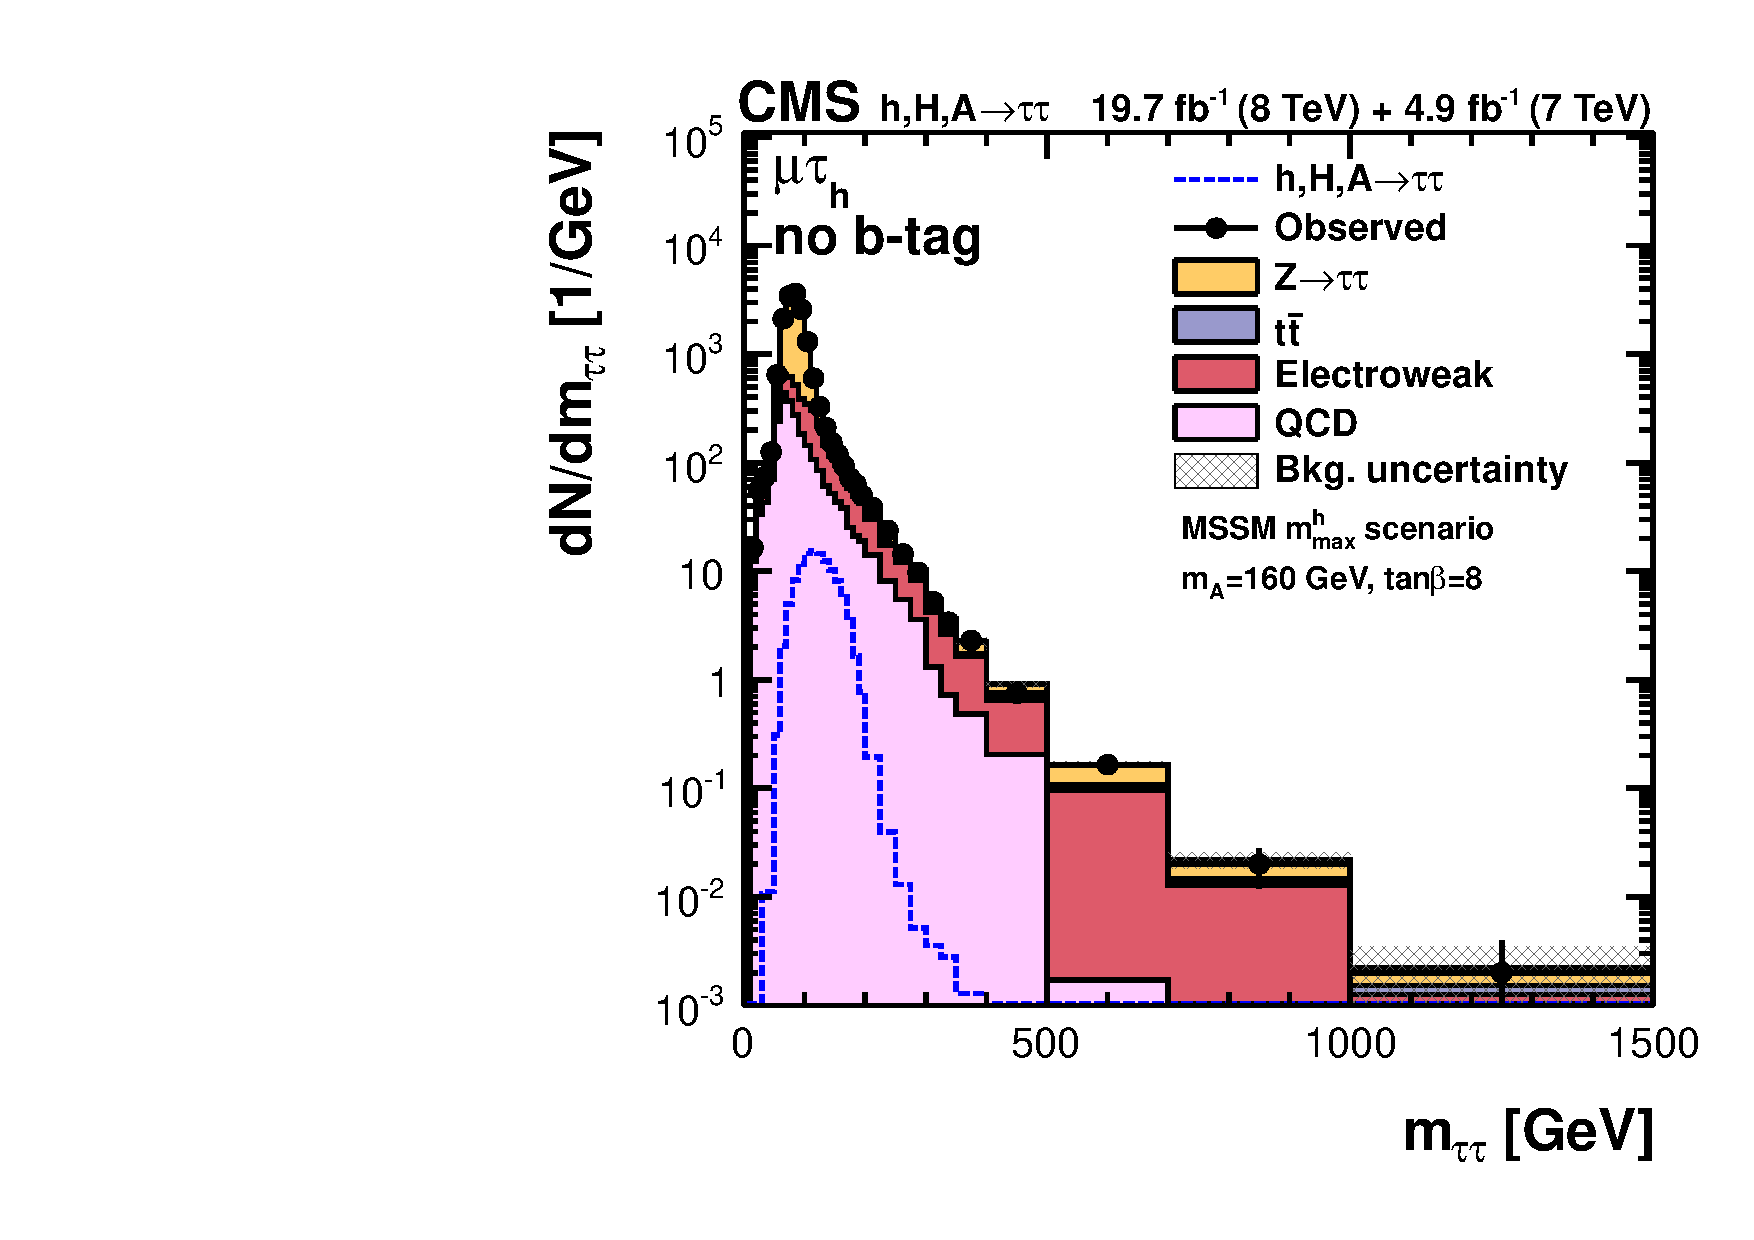
\includegraphics[width=0.5\textwidth]{plots/htt-mssm/muTau_nobtag_postfit_7TeV_8TeV_LOG.pdf}}
\subfloat[]{
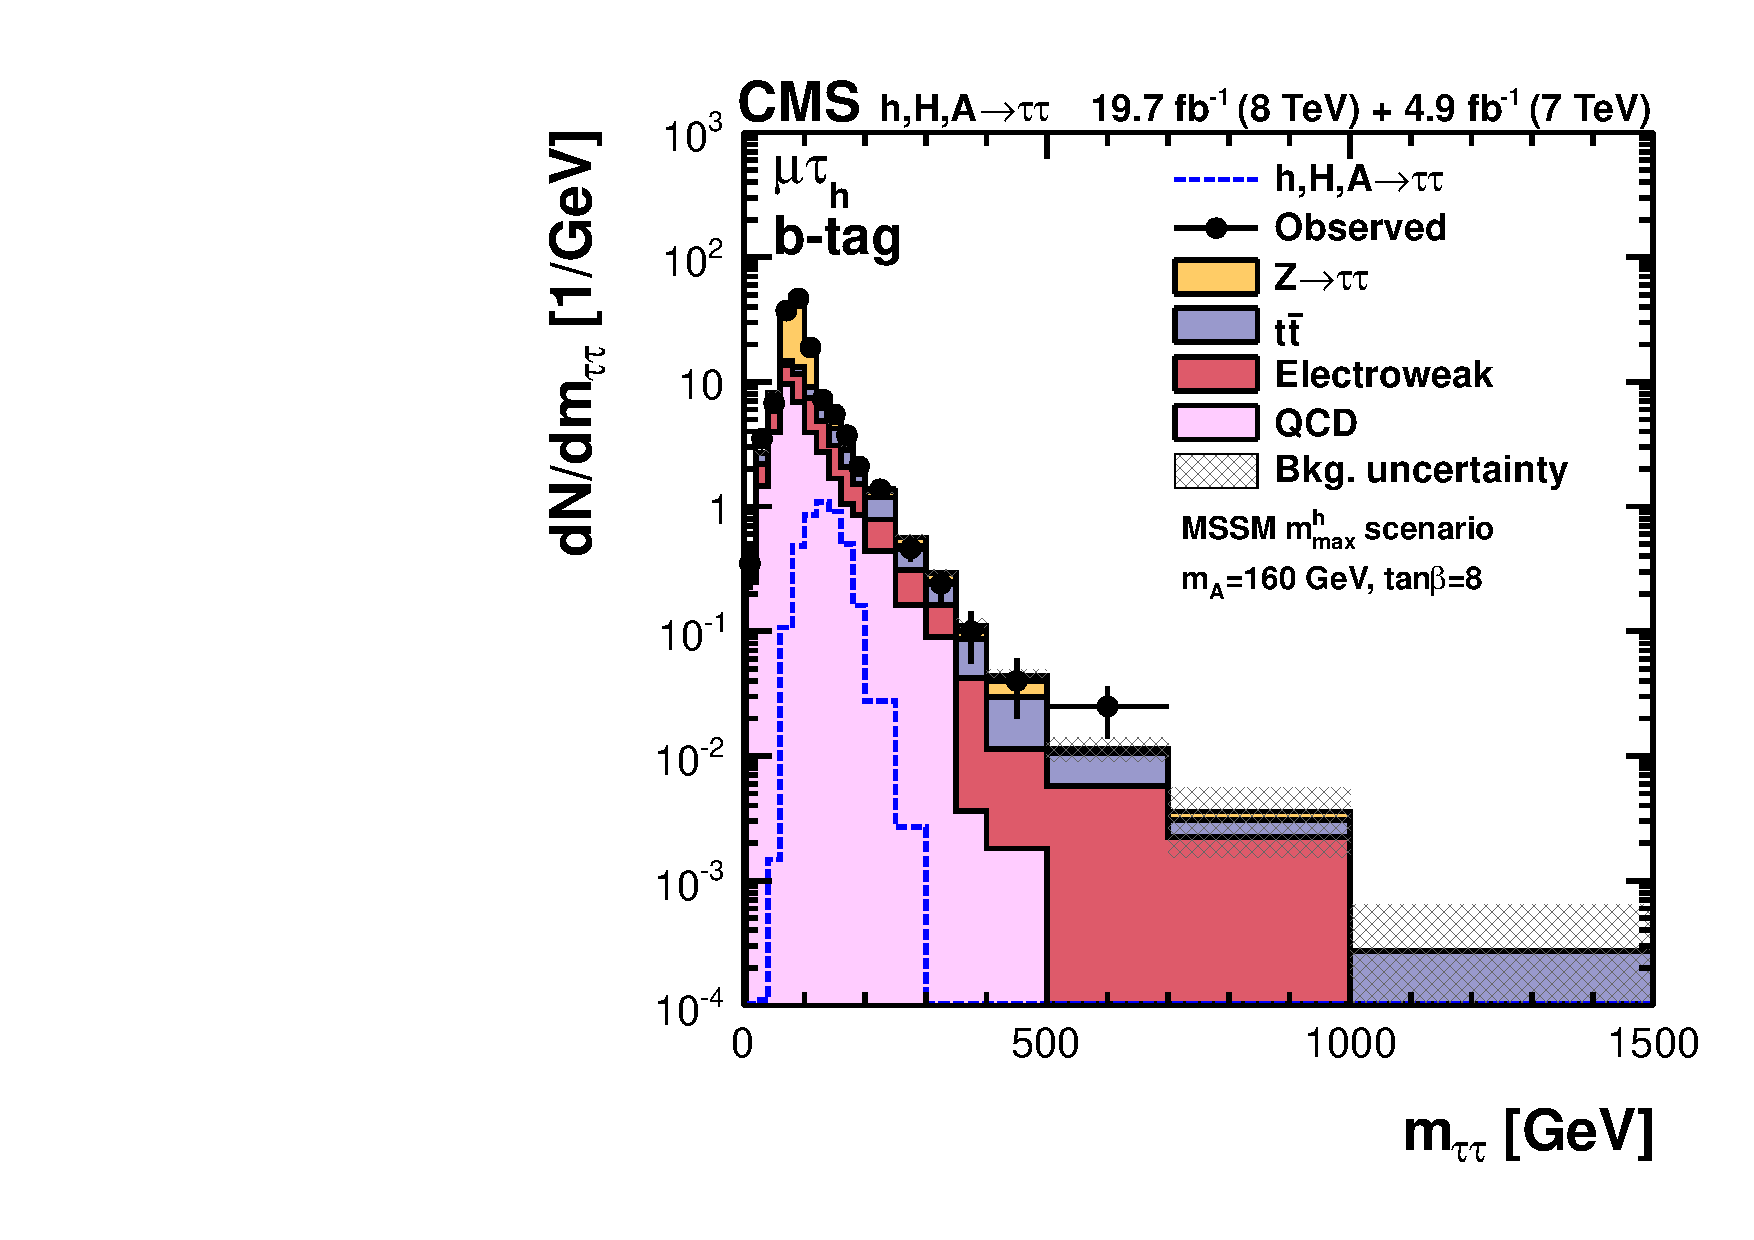
\includegraphics[width=0.5\textwidth]{plots/htt-mssm/muTau_btag_postfit_7TeV_8TeV_LOG.pdf}}

\subfloat[]{
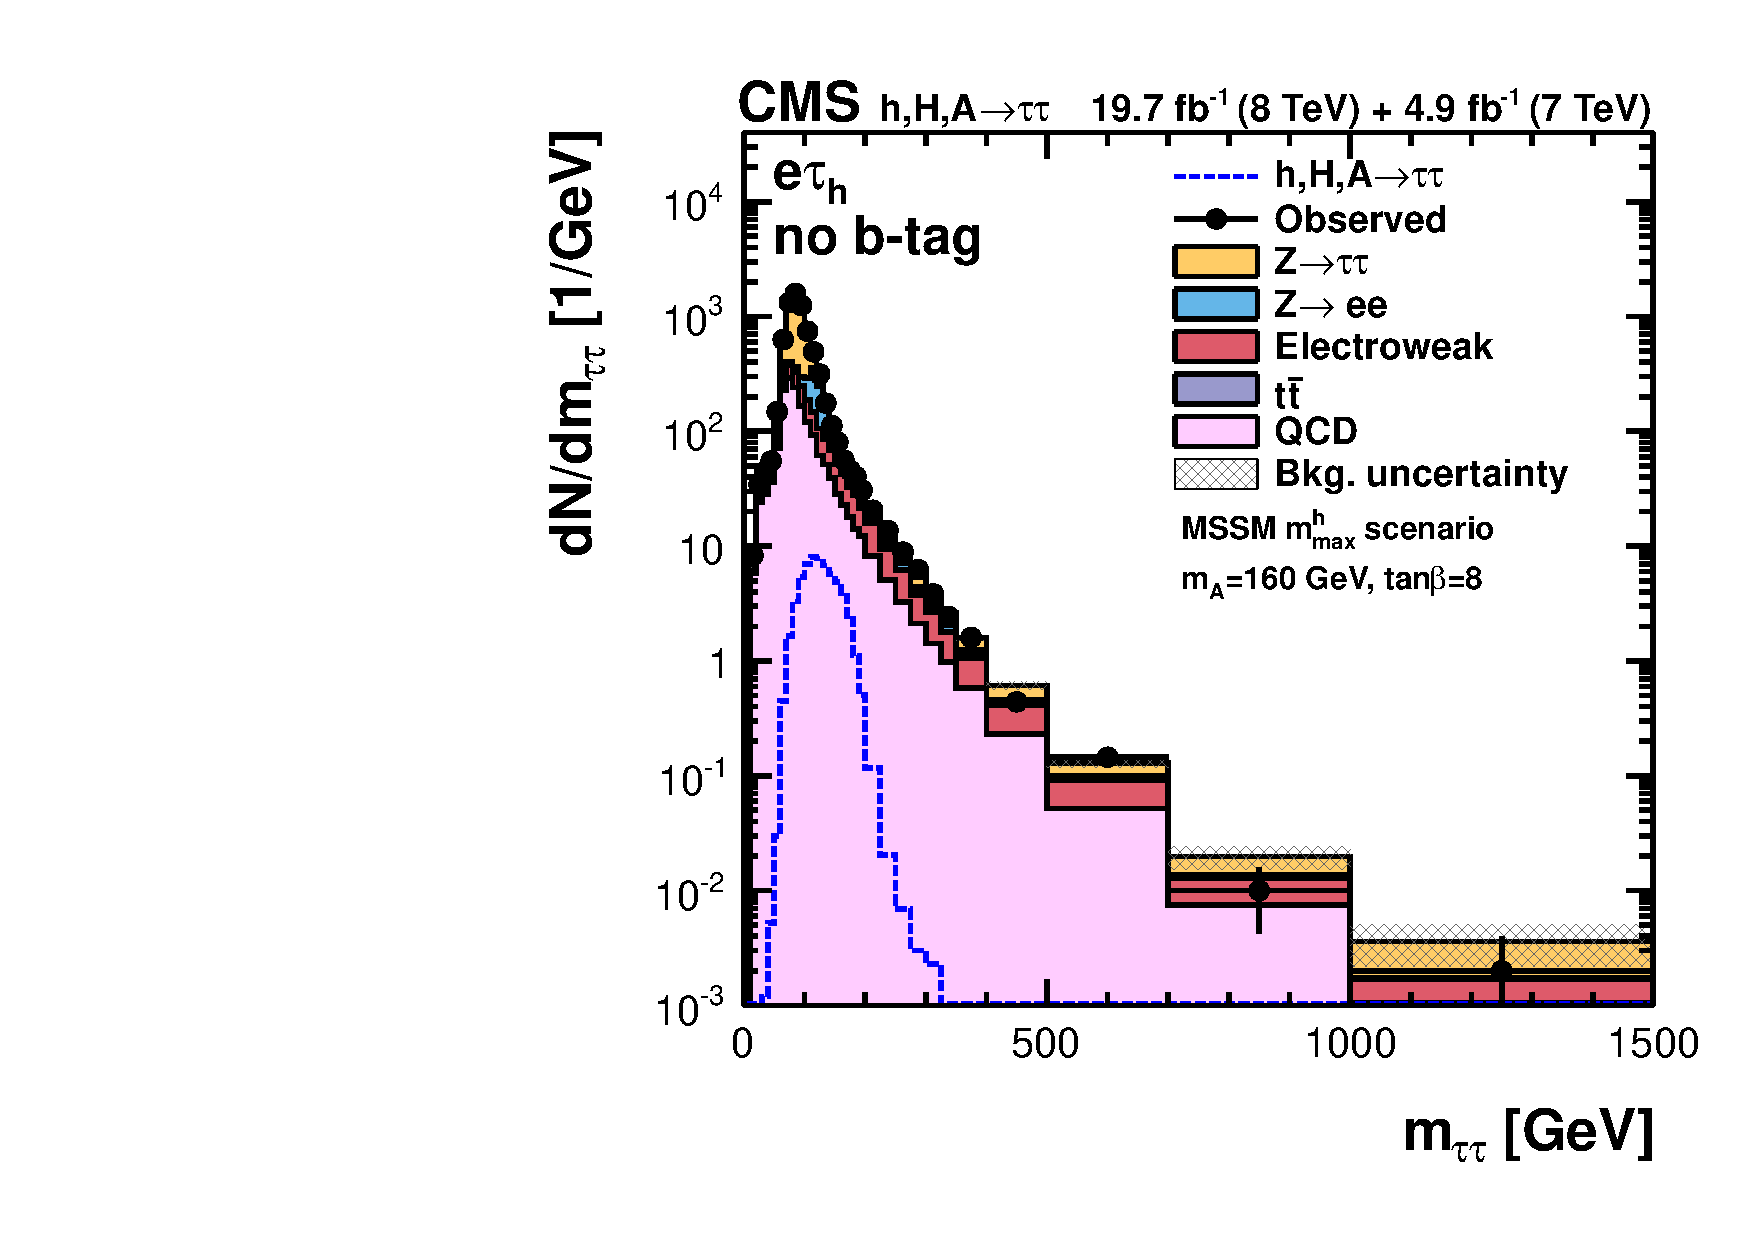
\includegraphics[width=0.5\textwidth]{plots/htt-mssm/eleTau_nobtag_postfit_7TeV_8TeV_LOG.pdf}}
\subfloat[]{
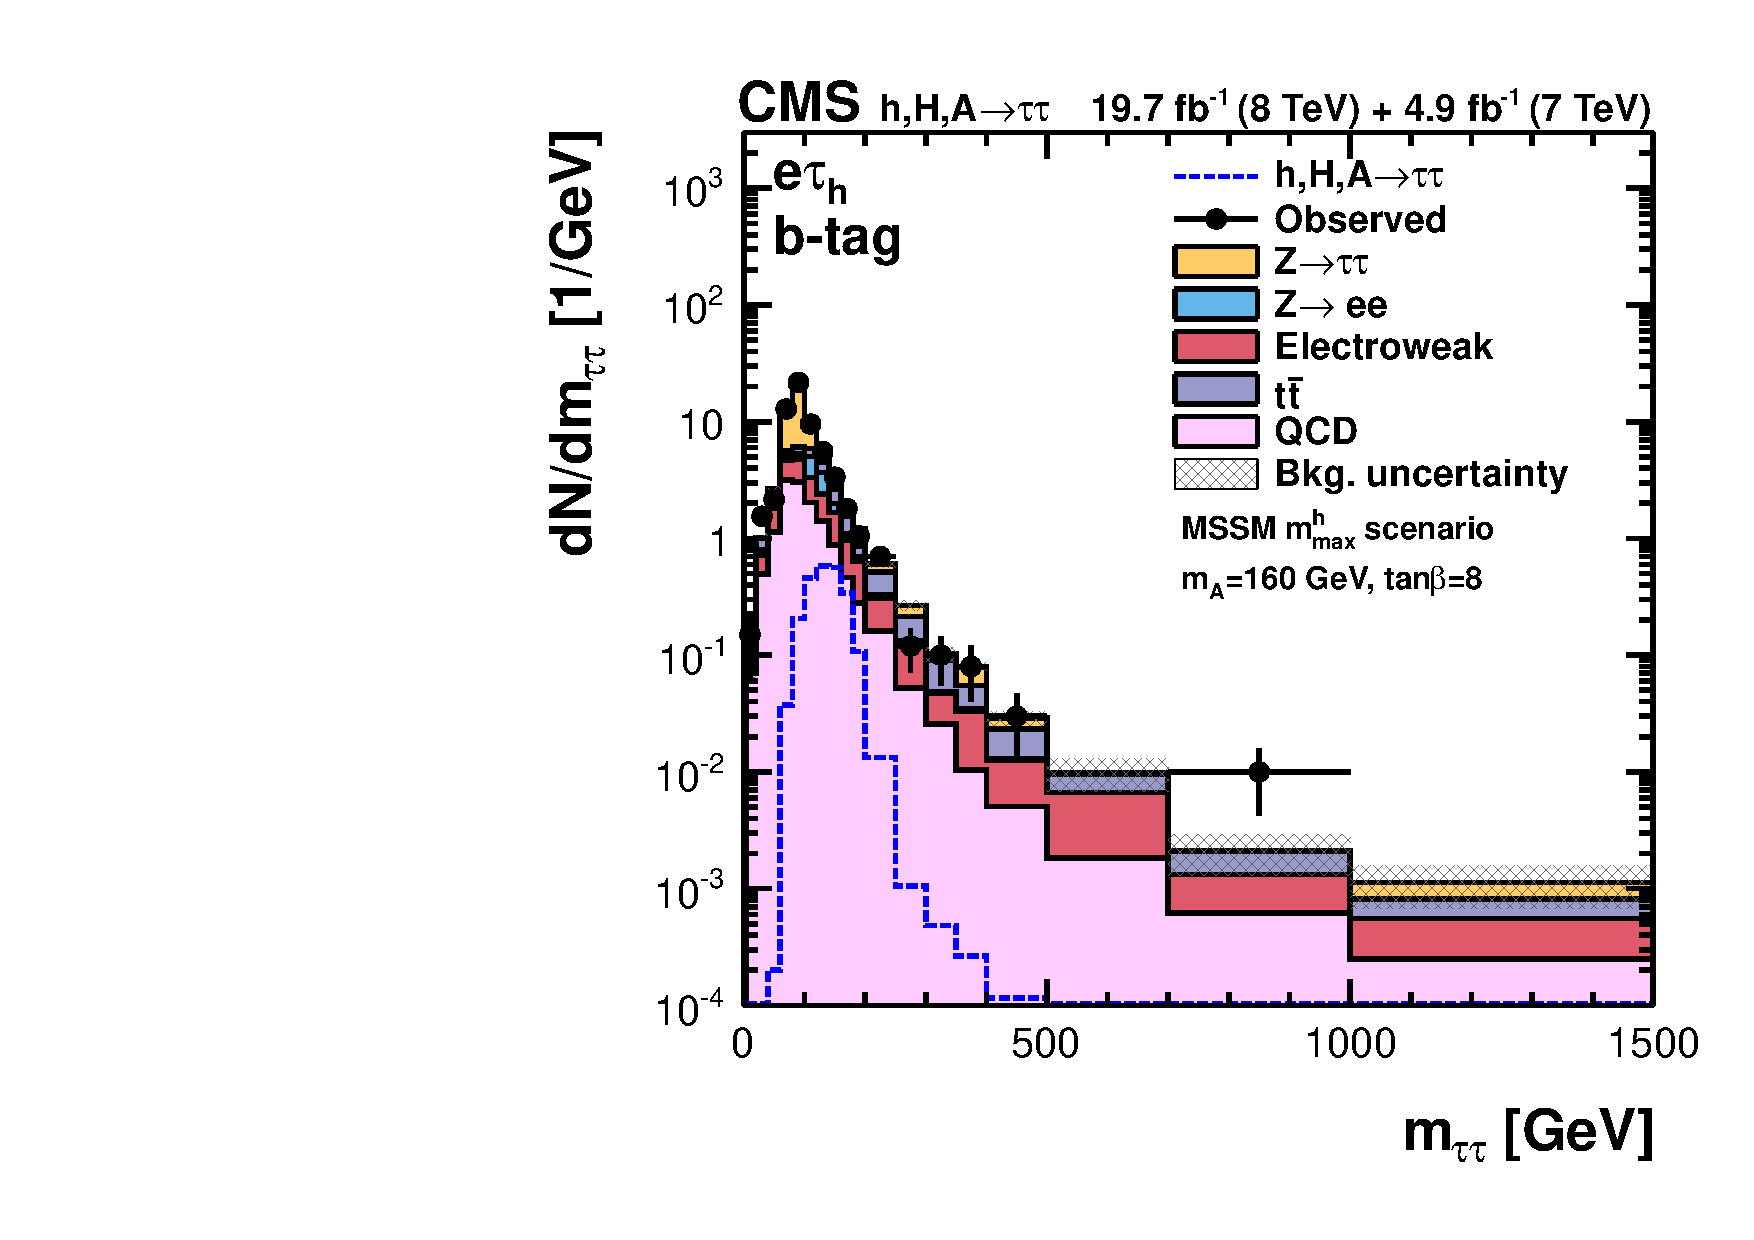
\includegraphics[width=0.5\textwidth]{plots/htt-mssm/eleTau_btag_postfit_7TeV_8TeV_LOG.pdf}}
\caption{Post-fit $m_{\Pgt\Pgt}$ distributions for the no-btag
(left) and b-tag categories. Plots are shown for
the $\mutau$ channel (top) and $\etau$ channel (bottom), for the combination of
7 and $8~\TeV$ data \cite{HIG-13-021}.}
\label{fig:mssmpostfitmass}
\end{figure}

The \ac{MSSM} analysis differs from the \ac{SM} analysis when we try to  
interpret the results of the maximum likelihood fit. This
is done differently for the two types of result producted - referred to as `model 
independent' and `model dependent'. 

\subsection{Model Independent Results}
\label{sec:modelindependent}

\subsubsection{2D Likelihood Scan}

As discussed in section~\ref{sec:signalextraction}, the maximum-likelihood fit
is generally performed in the signal plus background hypothesis, allowing the
signal to float as controlled by the signal strength modifier $\mu$. In the
\ac{SM} analysis the contributions from all different types of \ac{SM} Higgs
signal: gluon fusion, \ac{VBF} and associated production, are controlled by the
same $\mu$ which is normalised to the \ac{SM} predictions. For the \ac{MSSM}
analysis we have many alternative predictions for the cross-section times
branching ratio for each of the two productions processes: gluon fusion and
b-associated production, dependent on the choice of the parameters of the
\ac{MSSM} model. Hence we can use the maximum likelihood fit to obtain the best
choice of cross-section times branching ratio for each of the two production
processes from the fit to data, by letting them both float independently.

To do this we define our signal prediction as follows:
\begin{equation}
\mu \cdot s = \mu_{gg\Pphi} \cdot s_{gg\Pphi} + \mu_{bb\Pphi} \cdot s_{bb\Pphi} ,
\end{equation}

where $s_{gg\Pphi}$ and $s_{bb\Pphi}$ are the signal expectations for the gluon
fusion and b-associated production process and $\mu{gg\phi}$ and $\mu_{bb\phi}$
the signal strength modifiers. This can be directly inserted into the likelihood
term defined in equation~\ref{eq:LikelihoodFunction} to obtain a modified
likelihood which depends on two signal strength modifiers instead of one. A
likelihood scan is performed restricting the signal strength modifiers to both
be positive in steps of cross-section times branching ratio in picobarns. For
each point in the 2-D plane of the two signal strength modifiers, the negative
log likelihood, defined as:
\begin{equation}
NLL = - \ln \mathcal{L} ,  
\end{equation}
is evaluated. The lowest value of $NLL$ in the 2D plane is the best fit value
for the two signal strength modifiers. The one and two sigma contours are
calculated as the points $x$ in the plane where:

\begin{equation}
\Delta(NLL)_{1\sigma} = NLL(\text{best fit}) - NLL(x) = 0.5 ,\\ 
\Delta(NLL)_{2\sigma} = NLL(\text{best fit}) - NLL(x) = 1.92 ,\\ 
\end{equation}

where $NLL(\text{best fit})$ is the lowest $NLL$ value in the plane.

A likelihood scan is performed for each mass hypothesis $m_{\Pphi}$. Figure
\ref{fig:2Dlikelihood} shows the result for four sample mass points across the
plane. The best fit point is indicated by a black cross and the 1 and 2 $\sigma$
contours are shown. The fit result is compared with the result obtained in the
case where an \ac{SM} Higgs is in our dataset and no \ac{MSSM} Higgs is present
- this indicates that a small positive value of cross-section times branching
ratio for the gluon fusion production mode can be obtained as a result of the
\ac{SM} gluon fusion production.

\begin{figure}[tbh]
\subfloat[]{
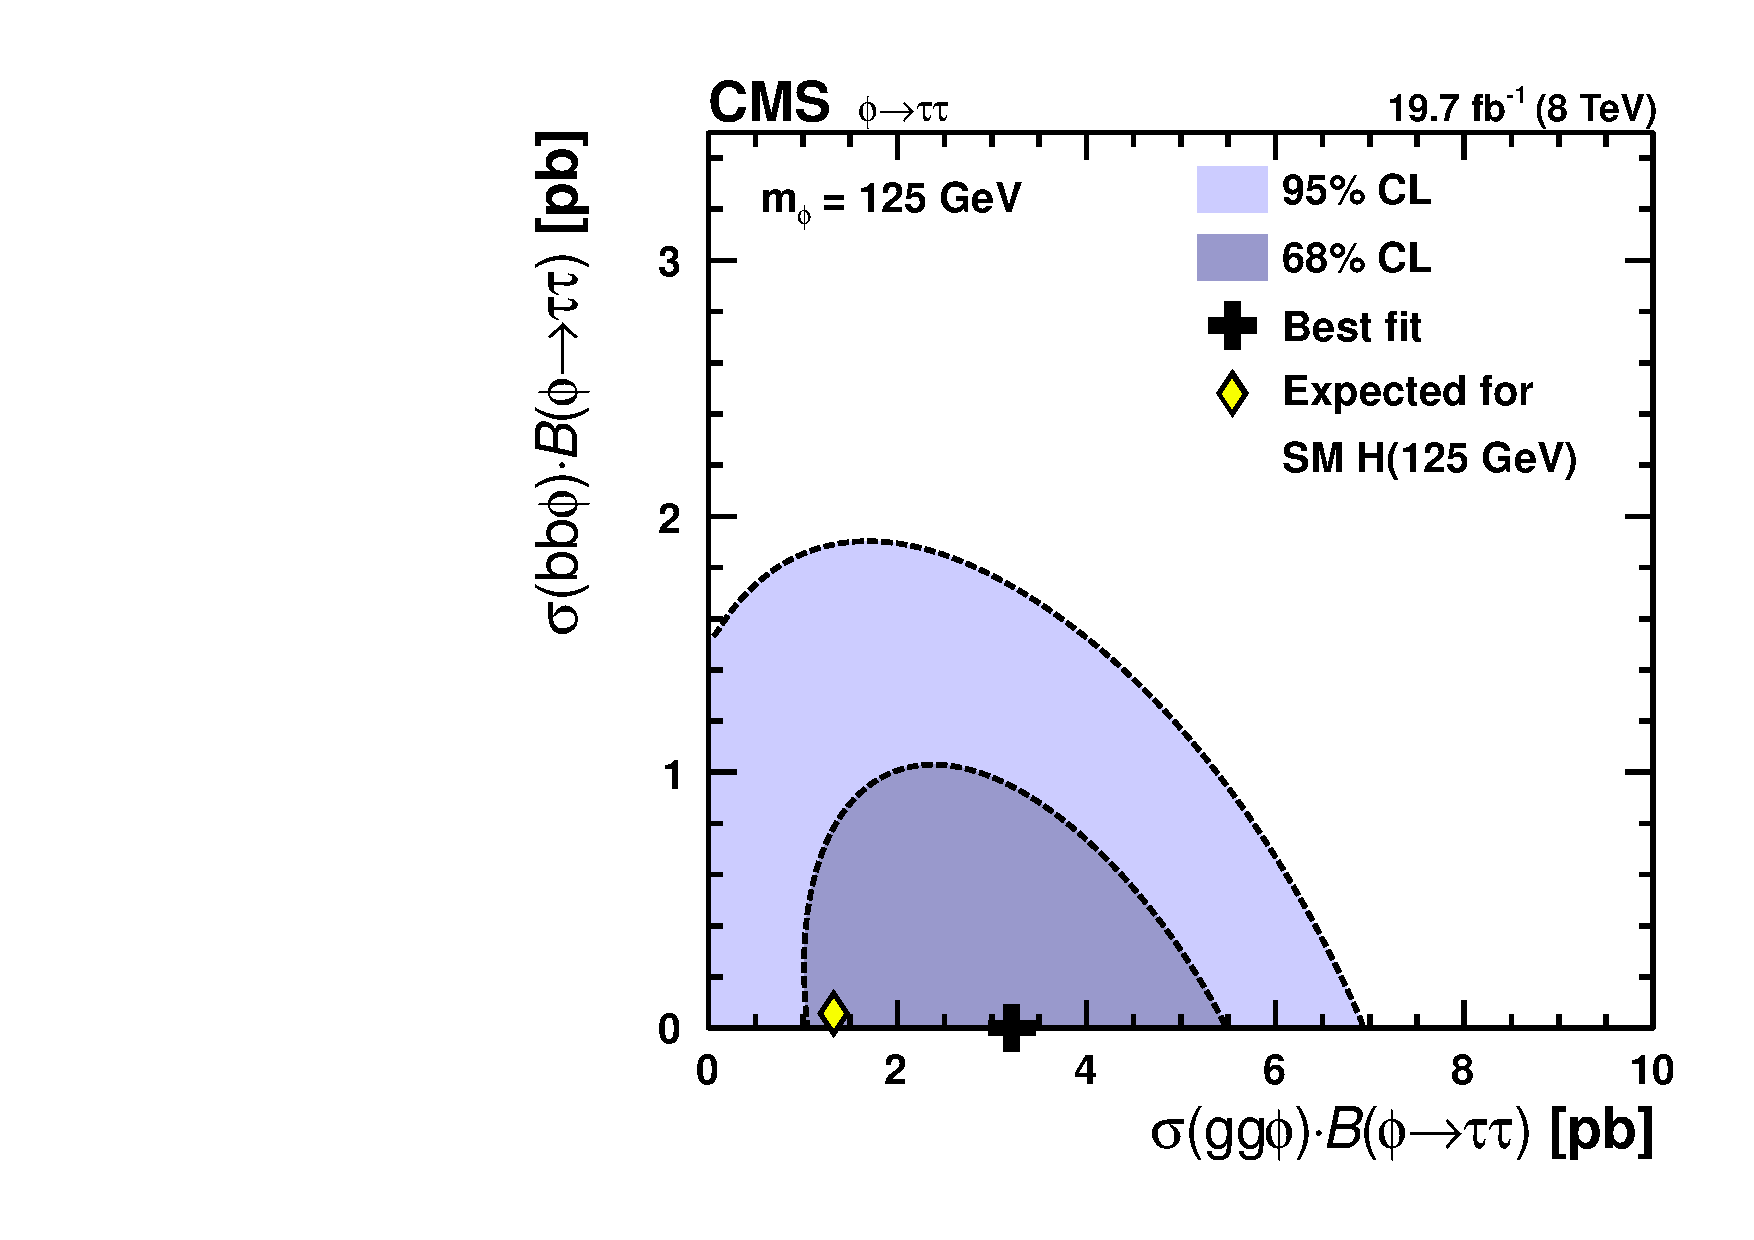
\includegraphics[width=0.5\textwidth]{plots/htt-mssm/bbb-ggH-bbH-scan-GGH-BBH-125.pdf}}
\subfloat[]{
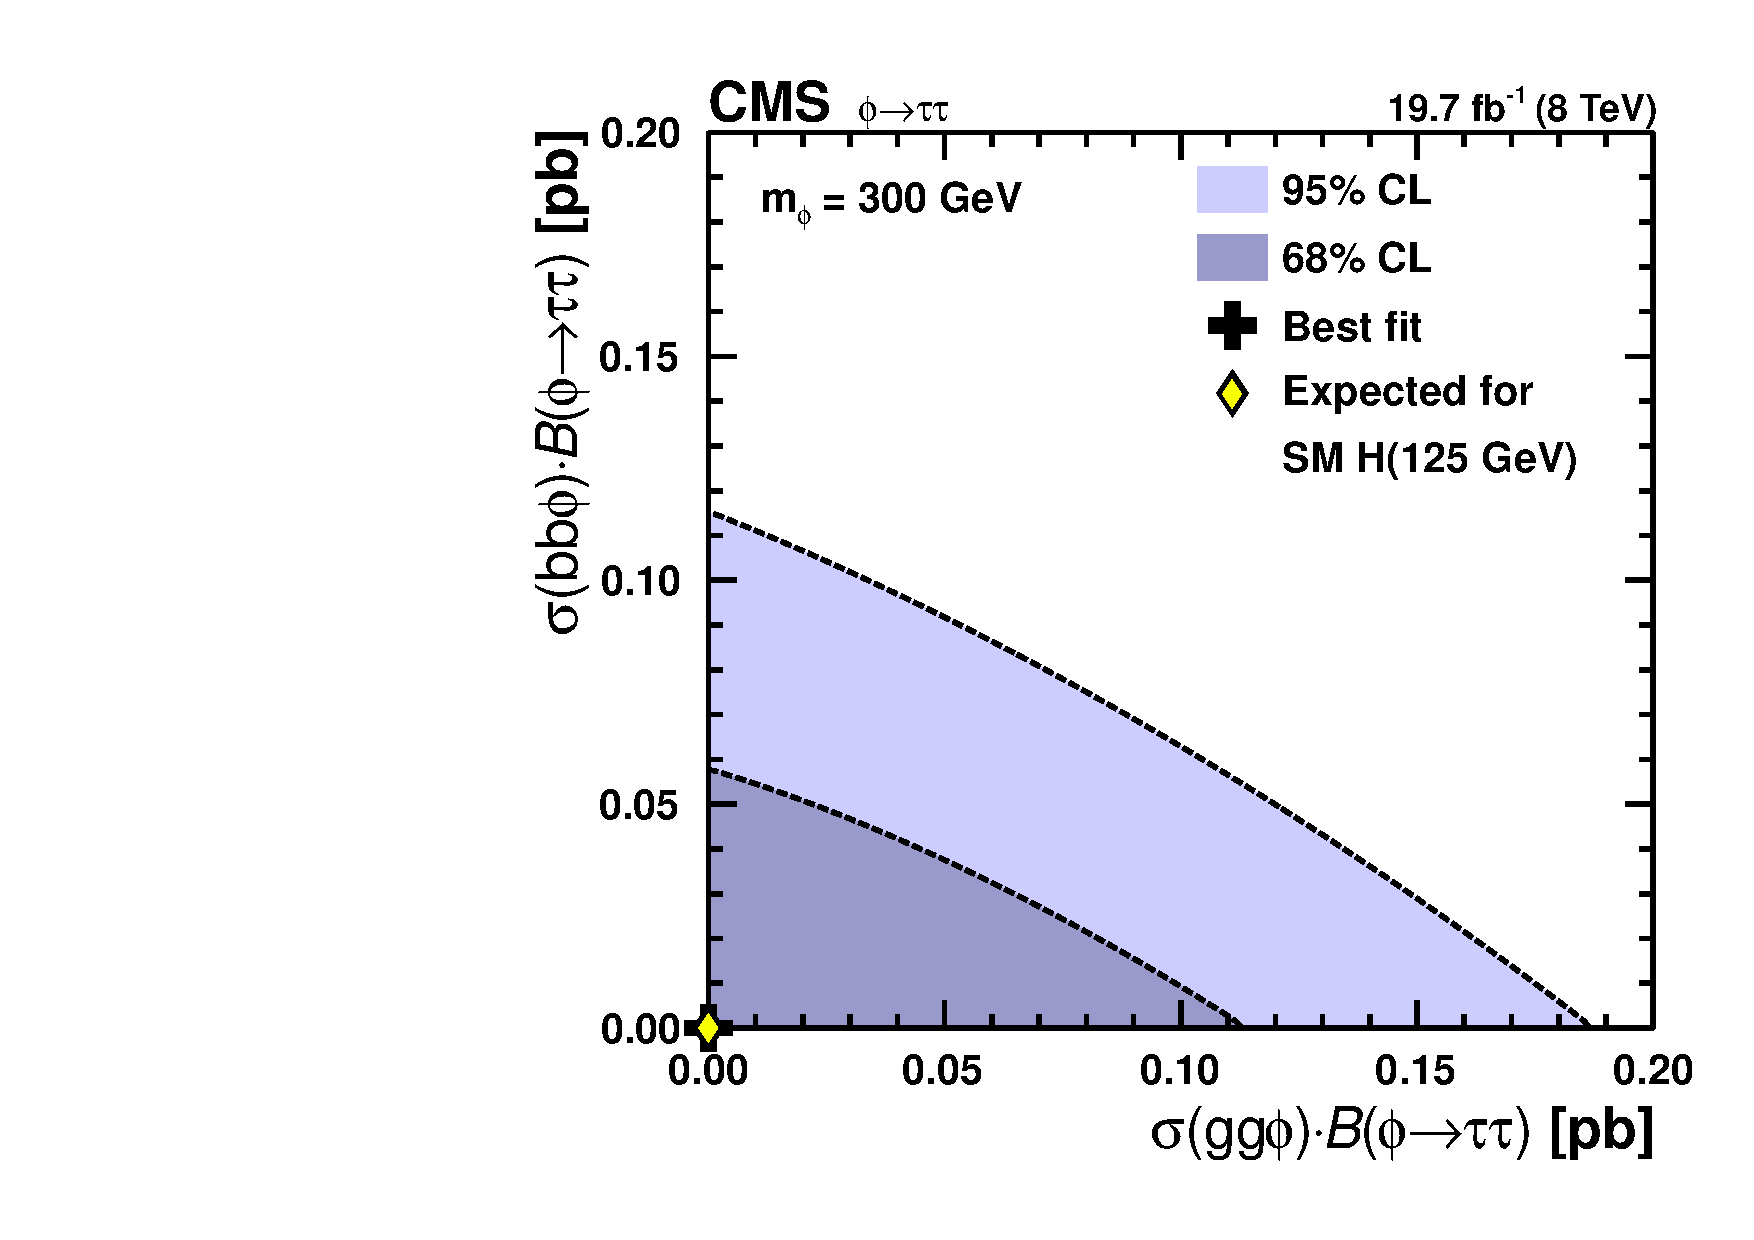
\includegraphics[width=0.5\textwidth]{plots/htt-mssm/bbb-ggH-bbH-scan-GGH-BBH-300.pdf}}

\subfloat[]{
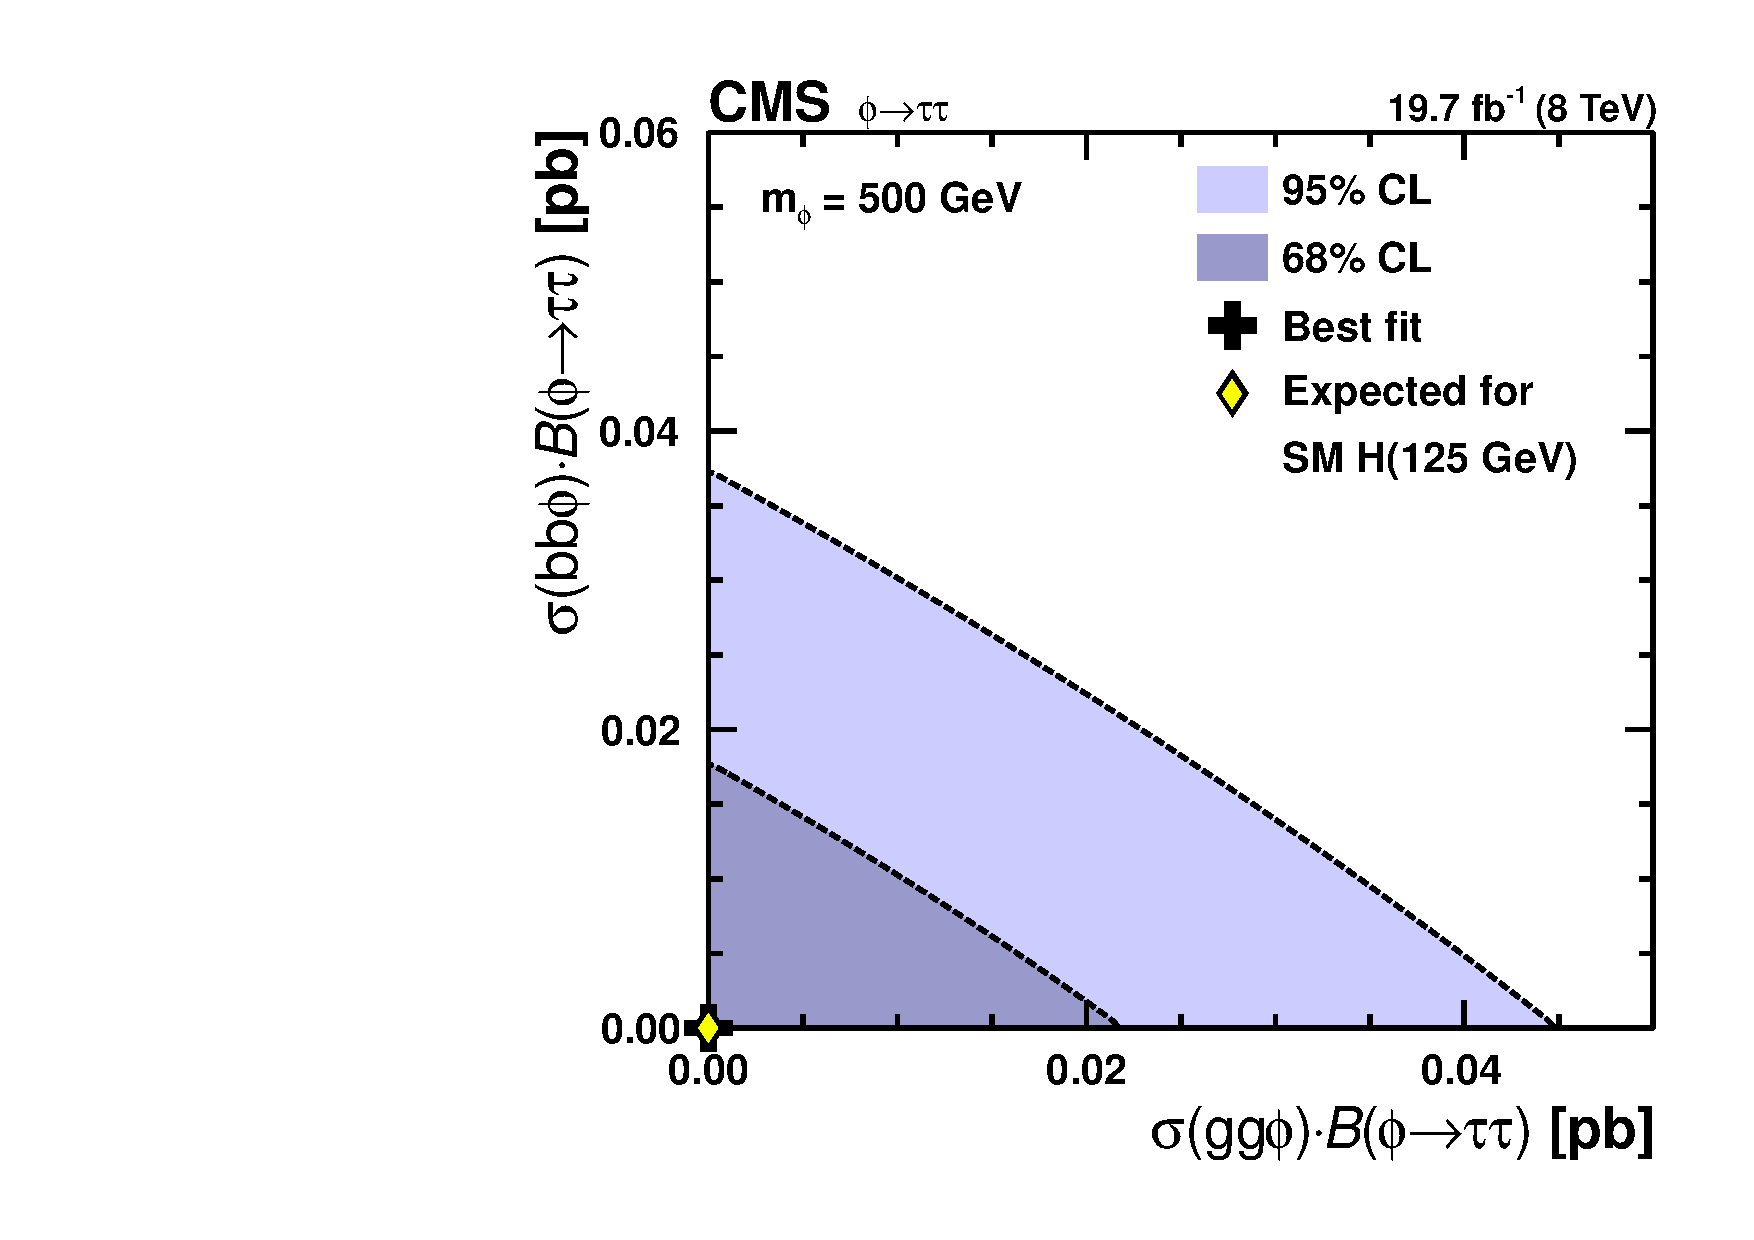
\includegraphics[width=0.5\textwidth]{plots/htt-mssm/bbb-ggH-bbH-scan-GGH-BBH-500.pdf}}
\subfloat[]{
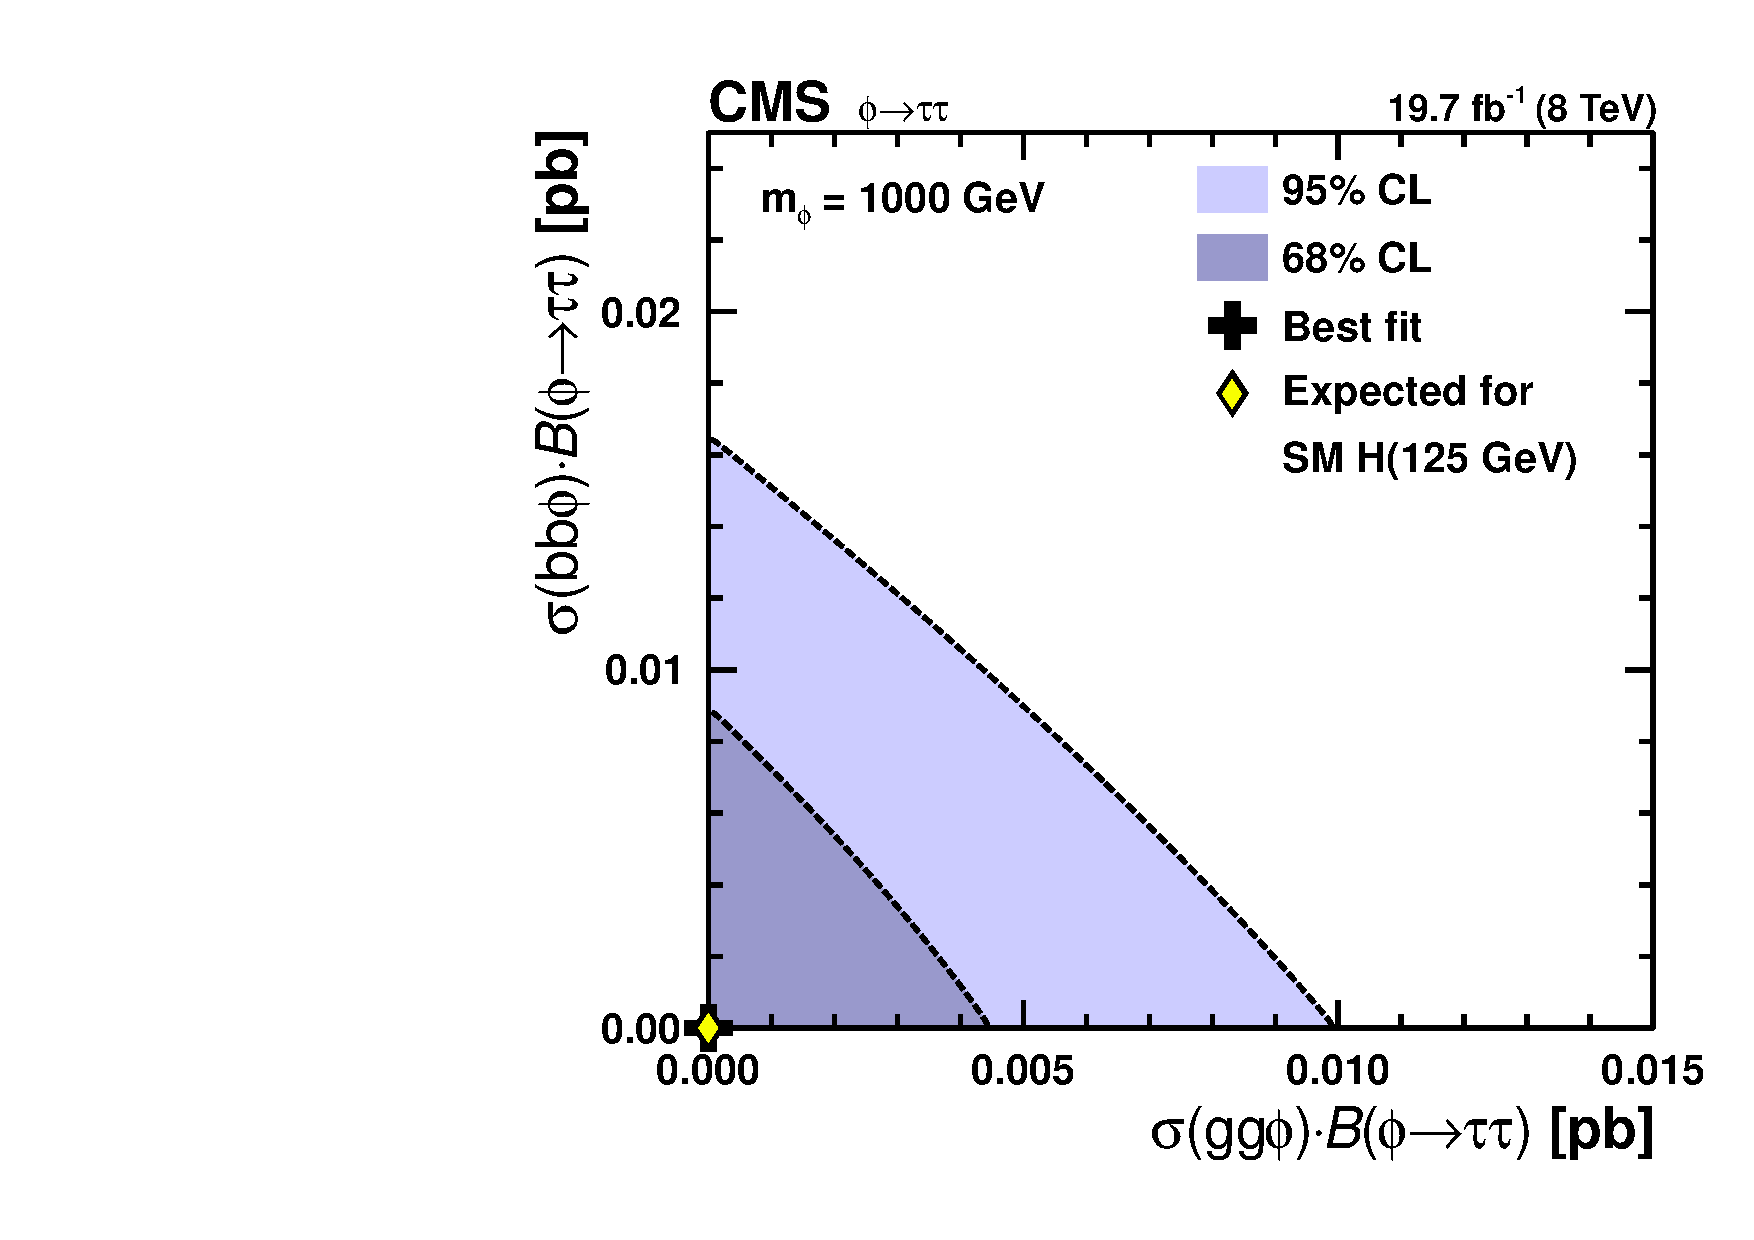
\includegraphics[width=0.5\textwidth]{plots/htt-mssm/bbb-ggH-bbH-scan-GGH-BBH-1000.pdf}}
\caption{2-D likelihood scans showing the best fit values for the cross-section
times branching ratio of the gluon fusion (x-axis) and b-assocated production
(y-axis) processes using 8~\TeV data. The best fit point is indicated along with the best fit
point which would be obtained if there was a 125~\GeV \ac{SM} Higgs boson in the data \cite{HIG-13-021}.}
\label{fig:2Dlikelihood}
\end{figure}


\subsubsection{Limits on $\sigma \times BR$}

The simplest type of limit produced in the \ac{MSSM} analysis is analogous to the 
expected limit on $\mu$ produced in the \ac{SM} analysis (figure
\ref{fig:results-limit}). In the \ac{MSSM} analysis, instead of setting a limit
on the signal strength modifier with reference to a benchmark cross-section, a
more 'model-independent' limit is given on cross-section times branching ratio
for the Higgs production process. This can then be interpreted in many different
benchmark models. A limit is set separately for each of the two dominant production modes,
b-associated production and gluon fusion production. It is not possible to
completely disentangle the two production modes - as shown in
section~\ref{sec:mssmEventSelection} the categorisation does not completely
separate the signal contributions, and some b-associated production signal is
found in no b--tag category and some gluon fusion in the b--tag category. Hence
to produce a limit on each process separately, the other signal process is
`profiled'. This means that it is allowed to float in the fit like the nuisance
parameters. This type of limit is referred to as a `single-resonance' search,
due to the fact that there is no requirement that the three Higgs bosons of the
\ac{MSSM} are included, the search is simply for the production of $\Pphi$,
which represents any of the three bosons.

Figure \ref{fig:mssmModelIndependent} shows the expected and observed limit on
cross-section times branching ratio for the gluon fusion and b-associated
production processes. The expected limit is generated in the same way as the
expected limit in figure \ref{results-limit} b), by injecting an \ac{SM} Higgs.
In this way the observed limit is compared to an expected including both the
backgrounds and an \ac{SM} Higgs. 

\begin{figure}[tbh]
\subfloat[]{
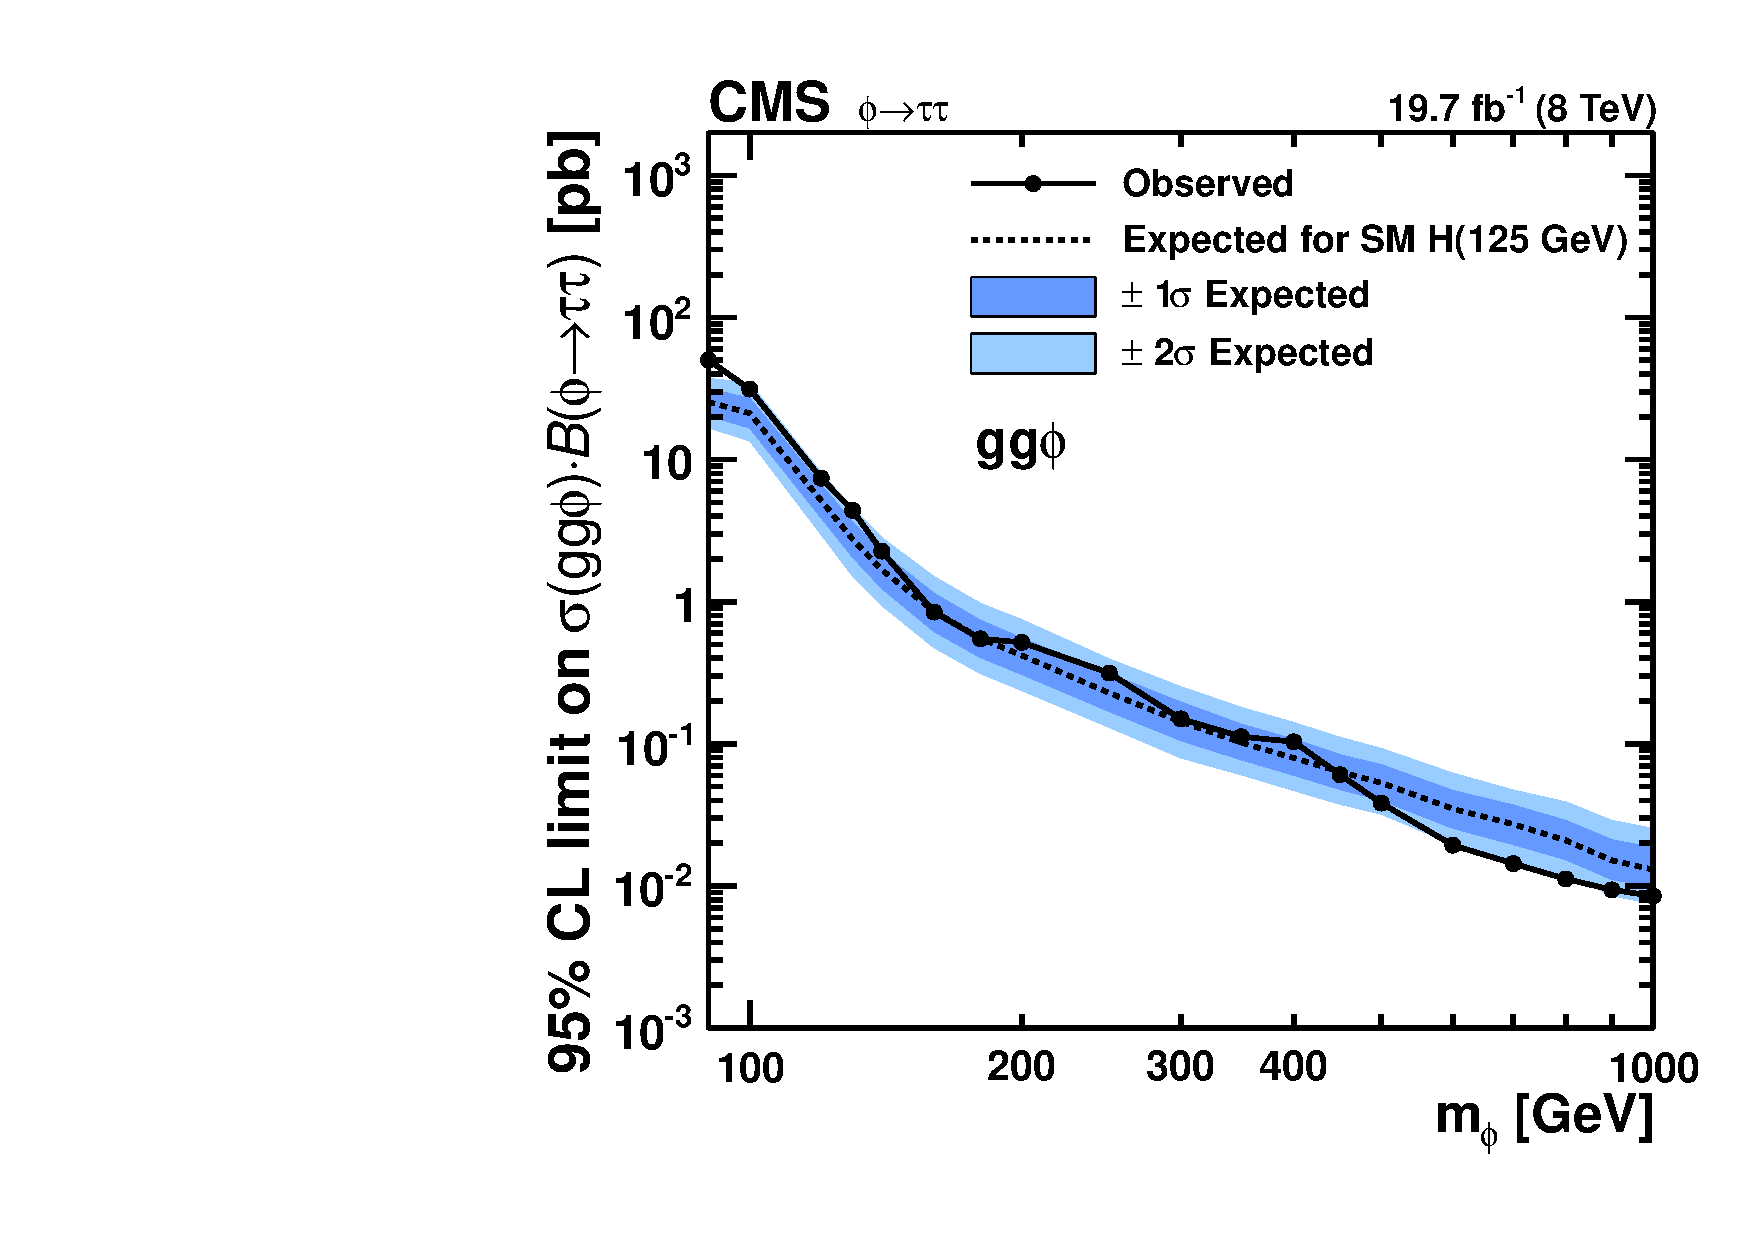
\includegraphics[width=0.5\textwidth]{plots/htt-mssm/cmb_ggH-limit.pdf}}
\subfloat[]{
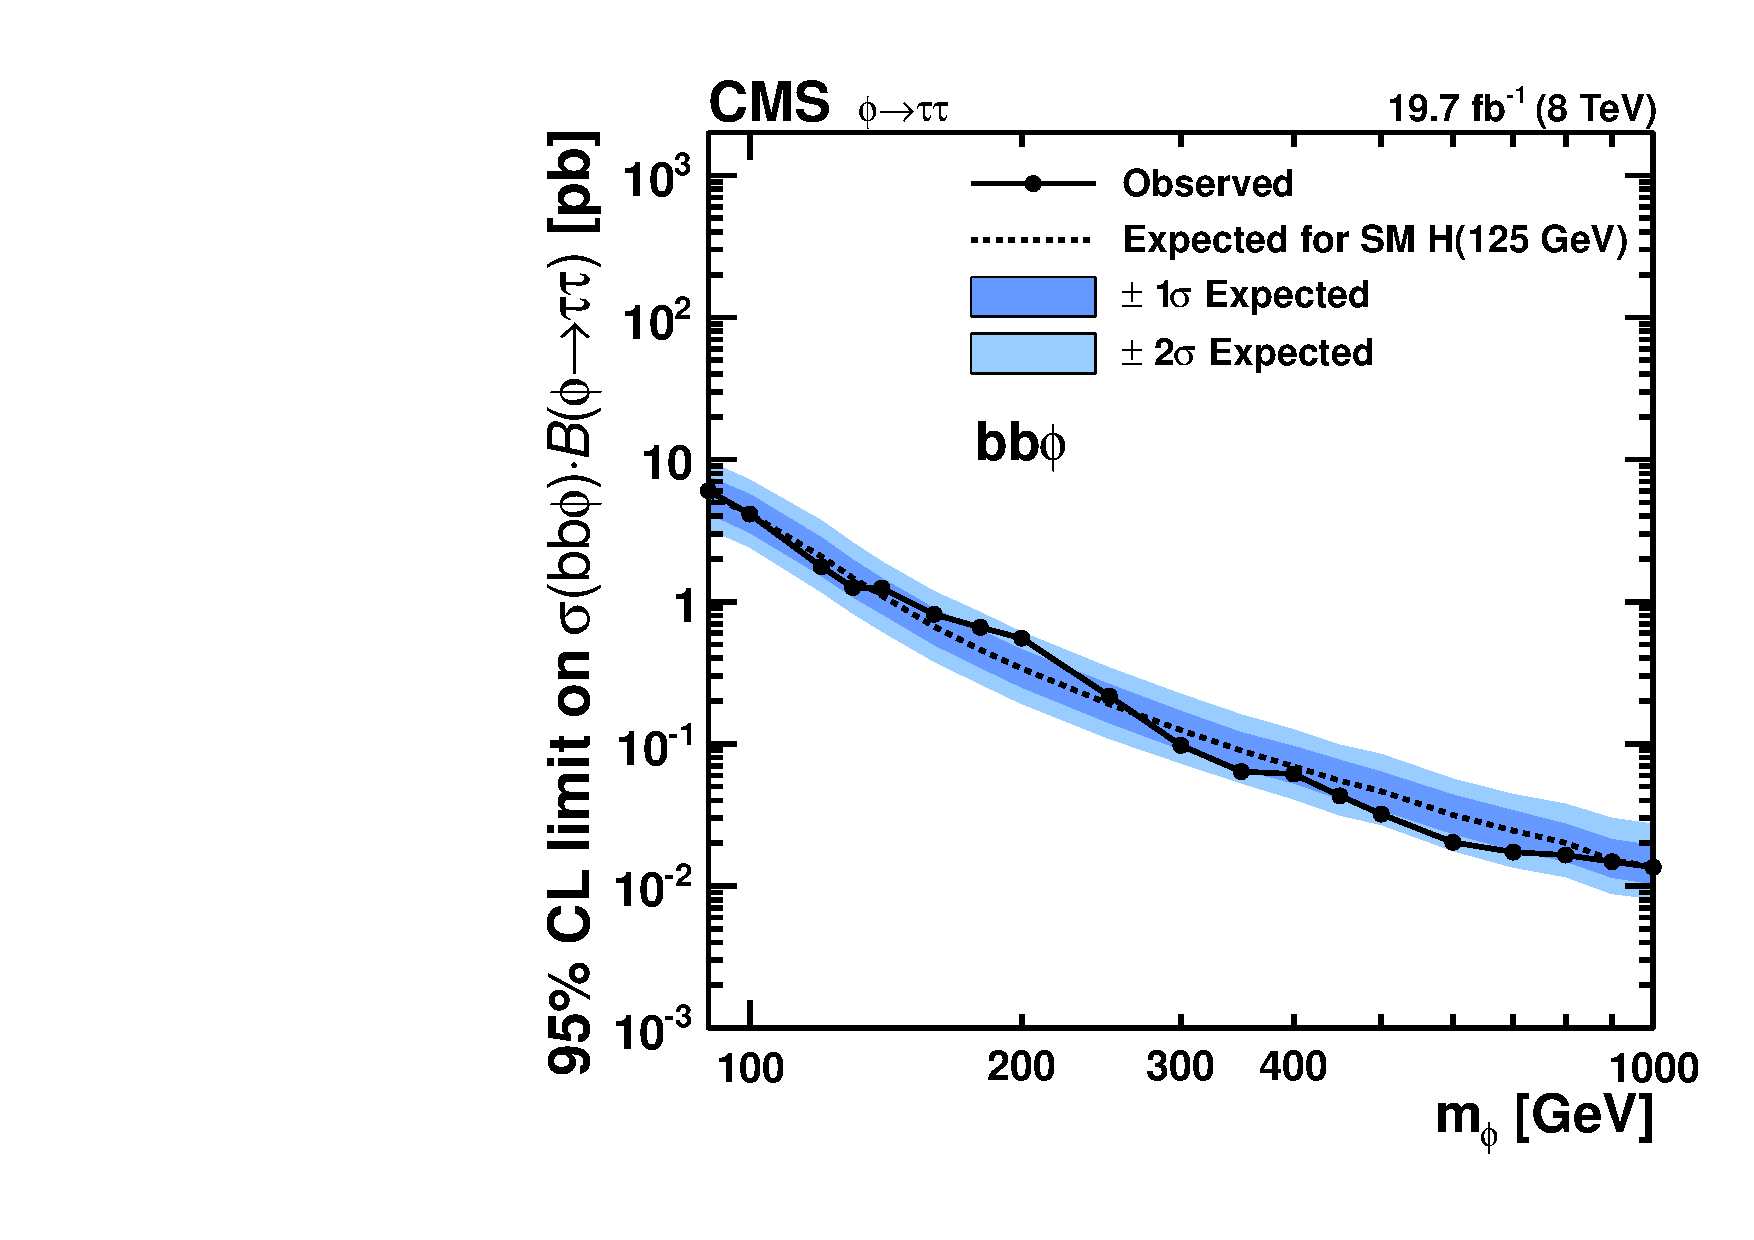
\includegraphics[width=0.5\textwidth]{plots/htt-mssm/cmb_bbH-limit.pdf}}
\caption{Limits on cross-section times branching ratio for a) gluon fusion Higgs
production and b) b-associated Higgs production for the combination of all
channels and categories. For each limit the other production process is
profiled. The observed limit is compared with an expected limit which includes
the \ac{SM} Higgs.}
\label{fig:mssmModelIndependent}
\end{figure}

The reason for comparing the observed with an expected including the \ac{SM} Higgs 
is that we cannot interpret results in the context of the \ac{MSSM} without taking into account
the fact that we have $3\sigma$ evidence of an \ac{SM}-like Higgs boson decaying
into taus. Despite the fact that the categorisation of events is chosen to
enhance selection of an \ac{MSSM} signal and not an \ac{SM} signal, the
selection is still very close to that of the \ac{SM} analysis and hence there is
still some sensitivity to the \ac{SM} Higgs in the \ac{MSSM} analysis. Thus we
have to interpret any excess in data over background very carefully, since it
does not automatically mean evidence of an \ac{MSSM} signal when it could be
from the \ac{SM} Higgs. 

\subsection{Model Dependent limits}
\label{sec:modeldependent}

The model independent results described in the previous section are open to
interpretation in a variety of models. It is also interesting to look more
closely at the interpretation of the results in particular benchmarks scenarios.
Such results are referred to as `model-dependent'. Model-dependent searches are
conducted in a plane of the two free parameters in the model, usually $m_{\PA}$
and $\tan\beta$. At each point in the phase space, the cross-section times
branching ratio for each of the three neutral Higgs bosons is calculated, taking
into account both production processes. The contribution of the three Higgs
bosons is then combined into one template. Hence, unlike in the
model-independent `single resonance' search, the consistency of the data with
all three Higgs bosons is considered. 

The sensitivity to the \ac{SM} Higgs becomes even more important in a
model-dependent result. As discussed in
section~\ref{sec:MSSMBenchmarks}, the \ac{MSSM} benchmark scenarios being tested in this
analysis are required to be consistent with experimental measurements of the
$125~\GeV$ Higgs bosons. Hence in such scenarios, one of the three neutral Higgs
bosons must be very similar to the \ac{SM} $125~\GeV$ Higgs boson. This means
that by construction an \ac{MSSM} signal from one of these benchmarks looks a
lot like the \ac{SM} signal, with the exception of the requirement of the
additional two Higgs bosons.

Hence when interpreting the results of the \ac{MSSM} search in the context of an
\ac{MSSM} benchmark scenario, it is not enough to simply construct a limit from
considering the background-only hypothesis compared with the
signal-plus-background hypothesis. Instead, we must build a limit based on
whether the data agrees better than the background plus \ac{SM} signal or
background plus \ac{MSSM} signal hypothesis.

\subsubsection{\ac{MSSM} and \ac{SM} hypothesis testing}

To compare two different signal hypotheses, the likelihood function as desribed
in equation~\ref{eq:LikelihoodFunction} must be modified. As described in the
text, this likelihood compares the observed data with an expected constructed as
$\mu \cdot s_{i}(\theta) + b_{i}(\theta)$. This must be modified to compare the data with the
following:
\begin{equation}
\mathcal{L}(\text{data} | \mu \cdot s_{i}(\theta) + b_{i}(\theta)) \rightarrow
\mathcal{L}(\text{data}|M(\mu,\theta)),
\end{equation}
with
\begin{equation}
M(\mu,\theta) = \mu \cdot s_{i}^{\text{MSSM}}(\theta) + (1-\mu) \cdot
s_{i}^{\text{SM}}(\theta) + b_{i}(\theta), 
\end{equation}

where $s_{i}^{\text{MSSM}}(\theta)$ and $s_{i}^{\text{SM}}(\theta)$ are the
signal expectations in the \ac{MSSM} and \ac{SM} hypotheses respectively. In
this likelihood the signal strength modifier $\mu$ connects both expectations,
with the null hypothesis being the \ac{SM} for $\mu=0$ and the alternative
hypothesis the \ac{MSSM} for $\mu=1$. 

With this likelihood, a slightly different form of the test statistic must be
built compared with that in equation~\ref{eq:ProfileLikelihood}. In the test
statistic used at the \ac{LHC}, the numerator is defined for some signal
strength $\mu$ compared with the signal strength which maxmises the likelihood,
$\hat{\mu}$. Here we instead want a version of the test statistic which tests
two fixed values of $\mu$ against on another. For this we use a test statistic
which was used at the Tevatron, and hence is referred to as the ``TEV'' test
statistic, which takes the general form:

\begin{equation}
%q_{0} = -2\ln ( \frac{\mathcal{L}(\text{data}|\mu\cdot s(\hat{\theta_{\mu}}) + b(\hat{\theta_{\mu}})) }
%{\mathcal{L}(\text{data}|b(\hat{\theta_{0}}))} )
q_{0} = -2\ln\frac{\mathcal{L}(\text{data}| \mu,\hat{\theta_{\mu}} ) }
{\mathcal{L}(\text{data}|\mu=0,\hat{\theta_{0}})}
\;\; \text{with the constraint} \; 0\leq\mu\, .
\end{equation}

In this test statistic a numerator corresponding to the signal strength $\mu$ is
compared with a denominator corresponding to $\mu=0$. Hence for form of this
test statistic for our hypothesis testing corresponds to the comparison between
$\mu=1$ and $\mu=0$, hence:

\begin{equation}
q_{\text{MSSMvsSM}} = -2\ln\frac{\mathcal{L}(\text{data}| M(1,\hat{\theta_{1}}) ) }
{\mathcal{L}(\text{data}| M(0,\hat{\theta_{0}}) )}.
\label{eq:qMSSMvsSM}
\end{equation}

The disadvantage of a test statistic of this type is that there is no asymptotic
approximation, and so the distributions of the probability distribution
functions for the test statistic must be generated using toys. Figure
\ref{fig:toydistribution} shows the distributions obtained using toys with
either the \ac{SM} or \ac{MSSM} signal hypothesis, and the observed value of the
test statistic is shown. For this example $m_{\PA}-\tan\beta$ point, it can be
seen that the separation between the two distributions is good, and hence this
point is able to be excluded in the absence of an excess. It can be seen that
the observed agrees better with the \ac{SM} hypothesis than the \ac{MSSM}
hypothesis, indicating the lack of such an excess. 

\begin{figure}[tbh]
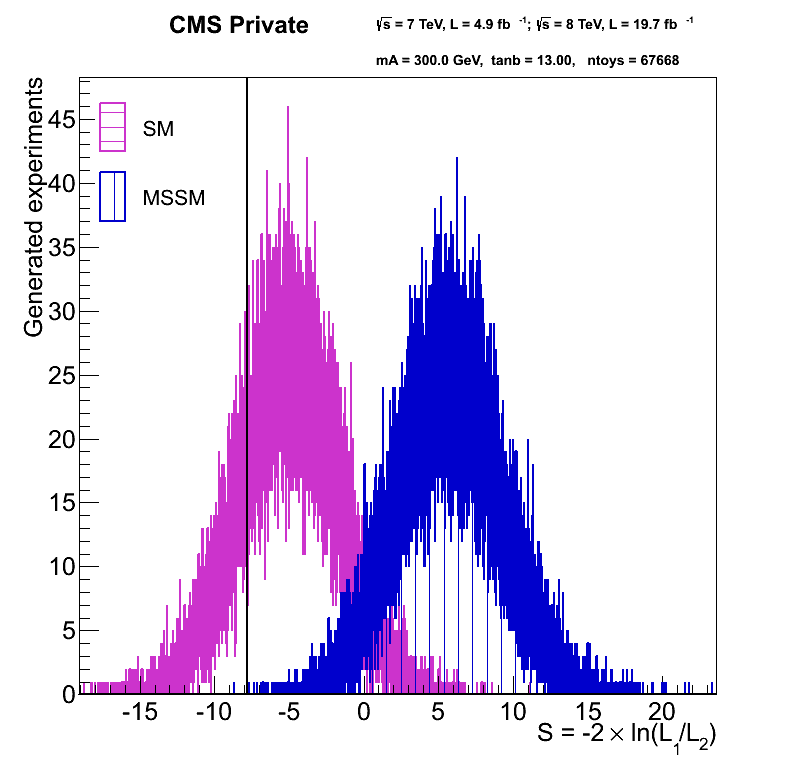
\includegraphics[width=0.7\textwidth]{plots/htt-mssm/sigsep_13.png}
\caption{Distributions of the test statistic for toys with \ac{MSSM} or \ac{SM}
signal for $m_{\PA} = 300~\GeV$, $\tan\beta = 13$ in the $m_{h}^{\text{max}}$
scenario. The black vertical line indictates the observed value of the test
statistic. The separation of the distributions is such that this point can be
excluded at 95$\%$ C.L.}
\label{fig:toydistribution}
\end{figure}

The CL$_{s}$ values are obtained using these probability distributions as
follows:

\begin{equation}
A = \int_{q_{0}^{x}}^{\infty}f(q_{0},\hat{\theta}_{0})\mathrm{d}q_{0}\, \\
B = \int_{q_{1}^{x}}^{\infty}f(q_{1},\hat{\theta}_{1})\mathrm{d}q_{1}\, \\
\mathrm{CL_{s}} = \frac{B}{A},
\end{equation}

where $x$ is either the 0.025, 0.16, 0.5, 0.84 or 0.975 quantile of the SM
probability density function (corresponding to -2$\sigma$, -1$\sigma$, expected,
$+1\sigma$, $+2\sigma$ exclusion) or the observed value. To obtain the final limit, 
a scan is performed in the two parameter plane and
the $\mathrm{CL_{s}}$ is calculated at each point in the grid. Each point is excluded at
95$\%$ C.L. if CL$_{s}<0.05$. A contour is drawn to connect the excluded points
using interpolation between neighbouring points in the grid.

Figure \ref{fig:hypotestcompare} shows the comparison between the exclusion
limits obtained using the conventional method of comparing \ac{MSSM} signal
hypothesis against background-only and using this new method to compare the
\ac{MSSM} and \ac{SM} hypotheses for the example of the $m_{\Ph}^\text{max}$
scenario. The left hand plot includes a line which shows
the effect of injecting an \ac{SM} signal into this limit. It can clearly be
seen that the effect of a possible \ac{SM} Higgs is not negligible and that a
possible excess in these plots could be the result of the \ac{SM} Higgs in our
dataset. In these results the data are consistent with both the background only
and the background plus \ac{SM} signal hypotheses.

\begin{figure}[tbh]
\subfloat[]{
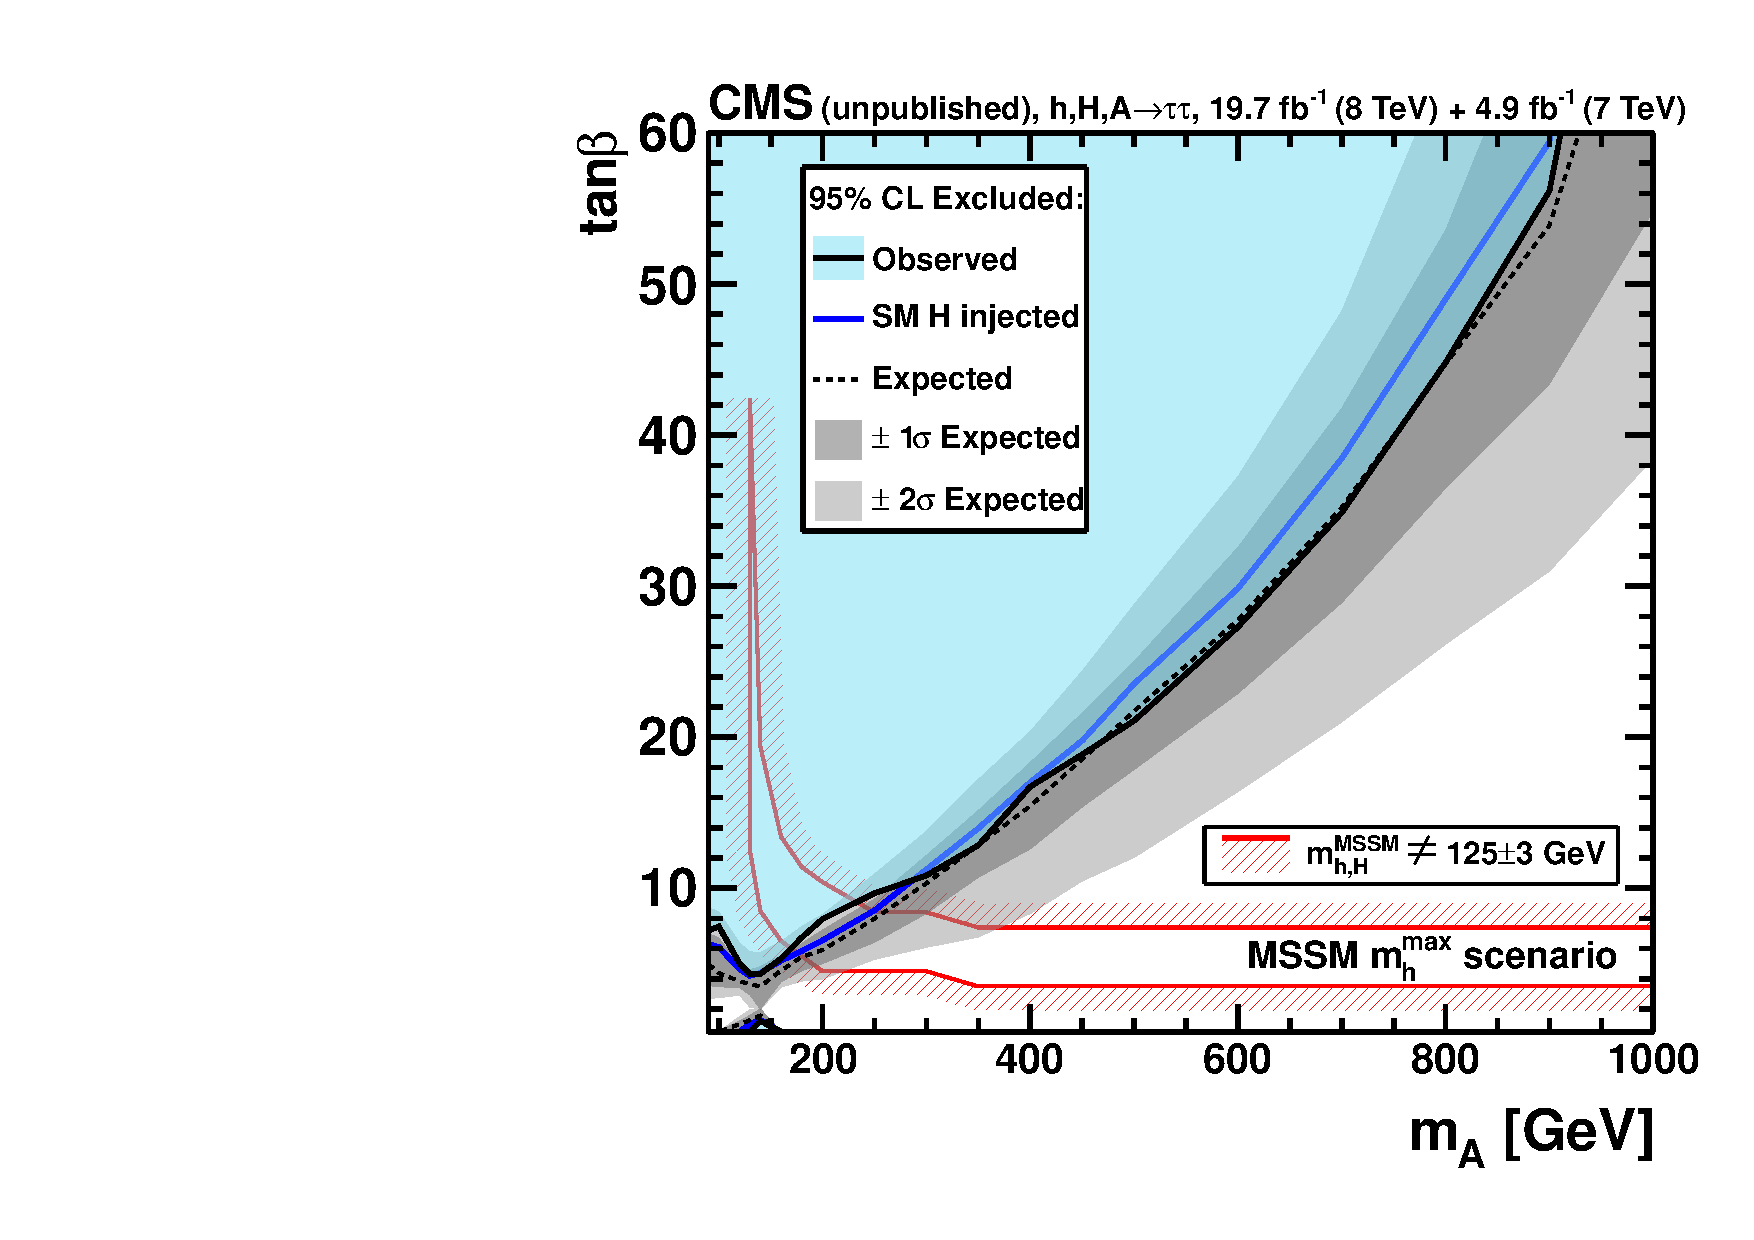
\includegraphics[width=0.5\textwidth]{plots/htt-mssm/cmb_mhmax-mA-tanb-SMinjected.pdf}}
\subfloat[]{
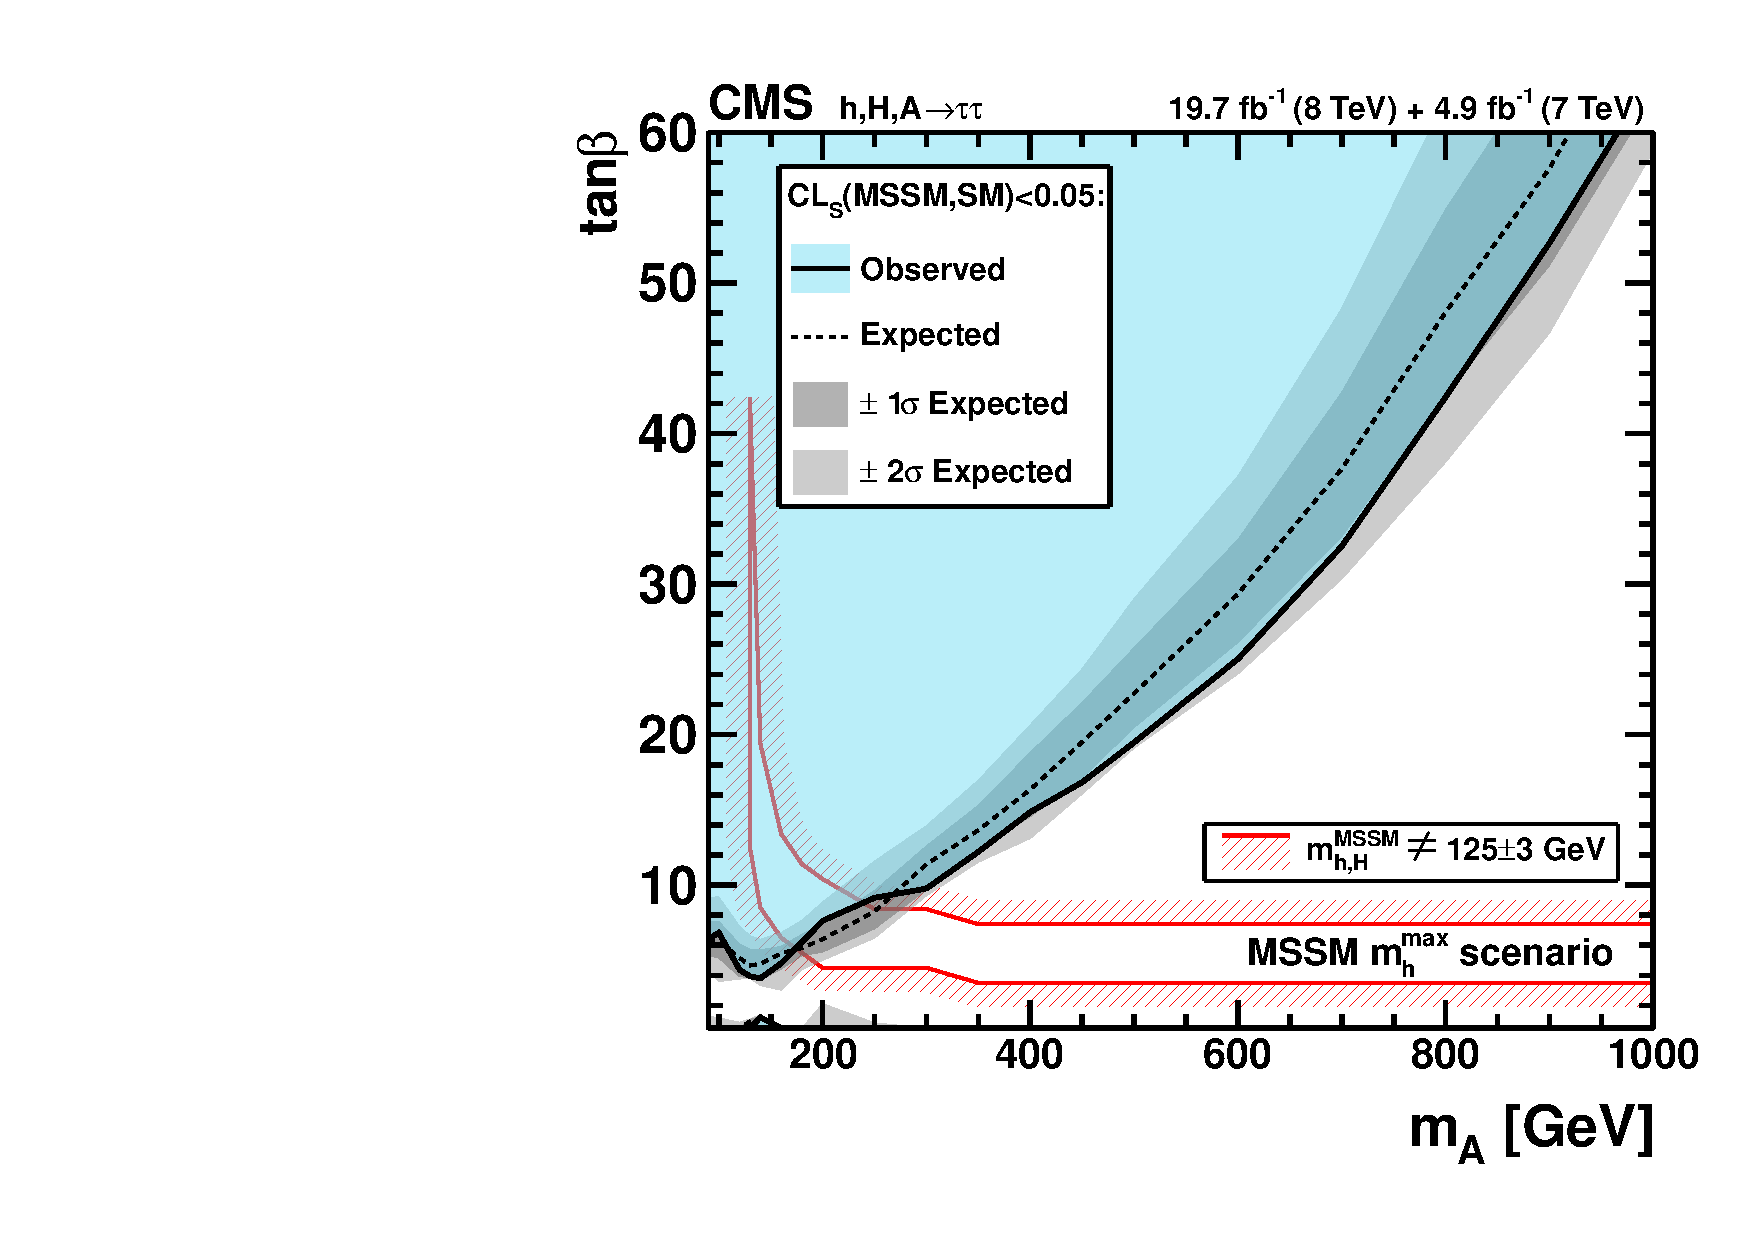
\includegraphics[width=0.5\textwidth]{plots/htt-mssm/cmbRL_mhmax-HypoTest.pdf}}
\caption{Expected and observed limit in the $m_{\PA}-\tan\beta$ plane of the
$m_H^{\text{max}}$ scenario. In the left hand plot, the \ac{MSSM} signal is
compared with the background only hypothesis. In the right hand plot, hypothesis
separation testing compares the \ac{MSSM} hypothesis with the \ac{SM}
hypothesis \cite{,HIG-13-021}.}
\label{fig:hypotestcompare}
\end{figure}


Note that the red areas indicated in figure \ref{fig:hypotestcompare} show the
region of phase space which is already ruled out by the constraint on the Higgs
mass being close to $125~\GeV$, with a $\pm 3~\GeV$ uncertainty due to
theoretical calculations in the \ac{MSSM}. The $m_{\Ph}^{\text{max}}$ scenario
is almost entirely ruled out by this constraint, as discussed in
section~\ref{sec:}. Figures \ref{fig:mhmodpmhmodm} to \ref{fig:tauphobiclowmH}
show the result interpreted in newer scenarios which better incorporate a
$125~\GeV$ Higgs. Large areas of the phase space in these scenarios is ruled out
by the lack of an excess in this analysis.


\begin{figure}[tbh]
\subfloat[]{
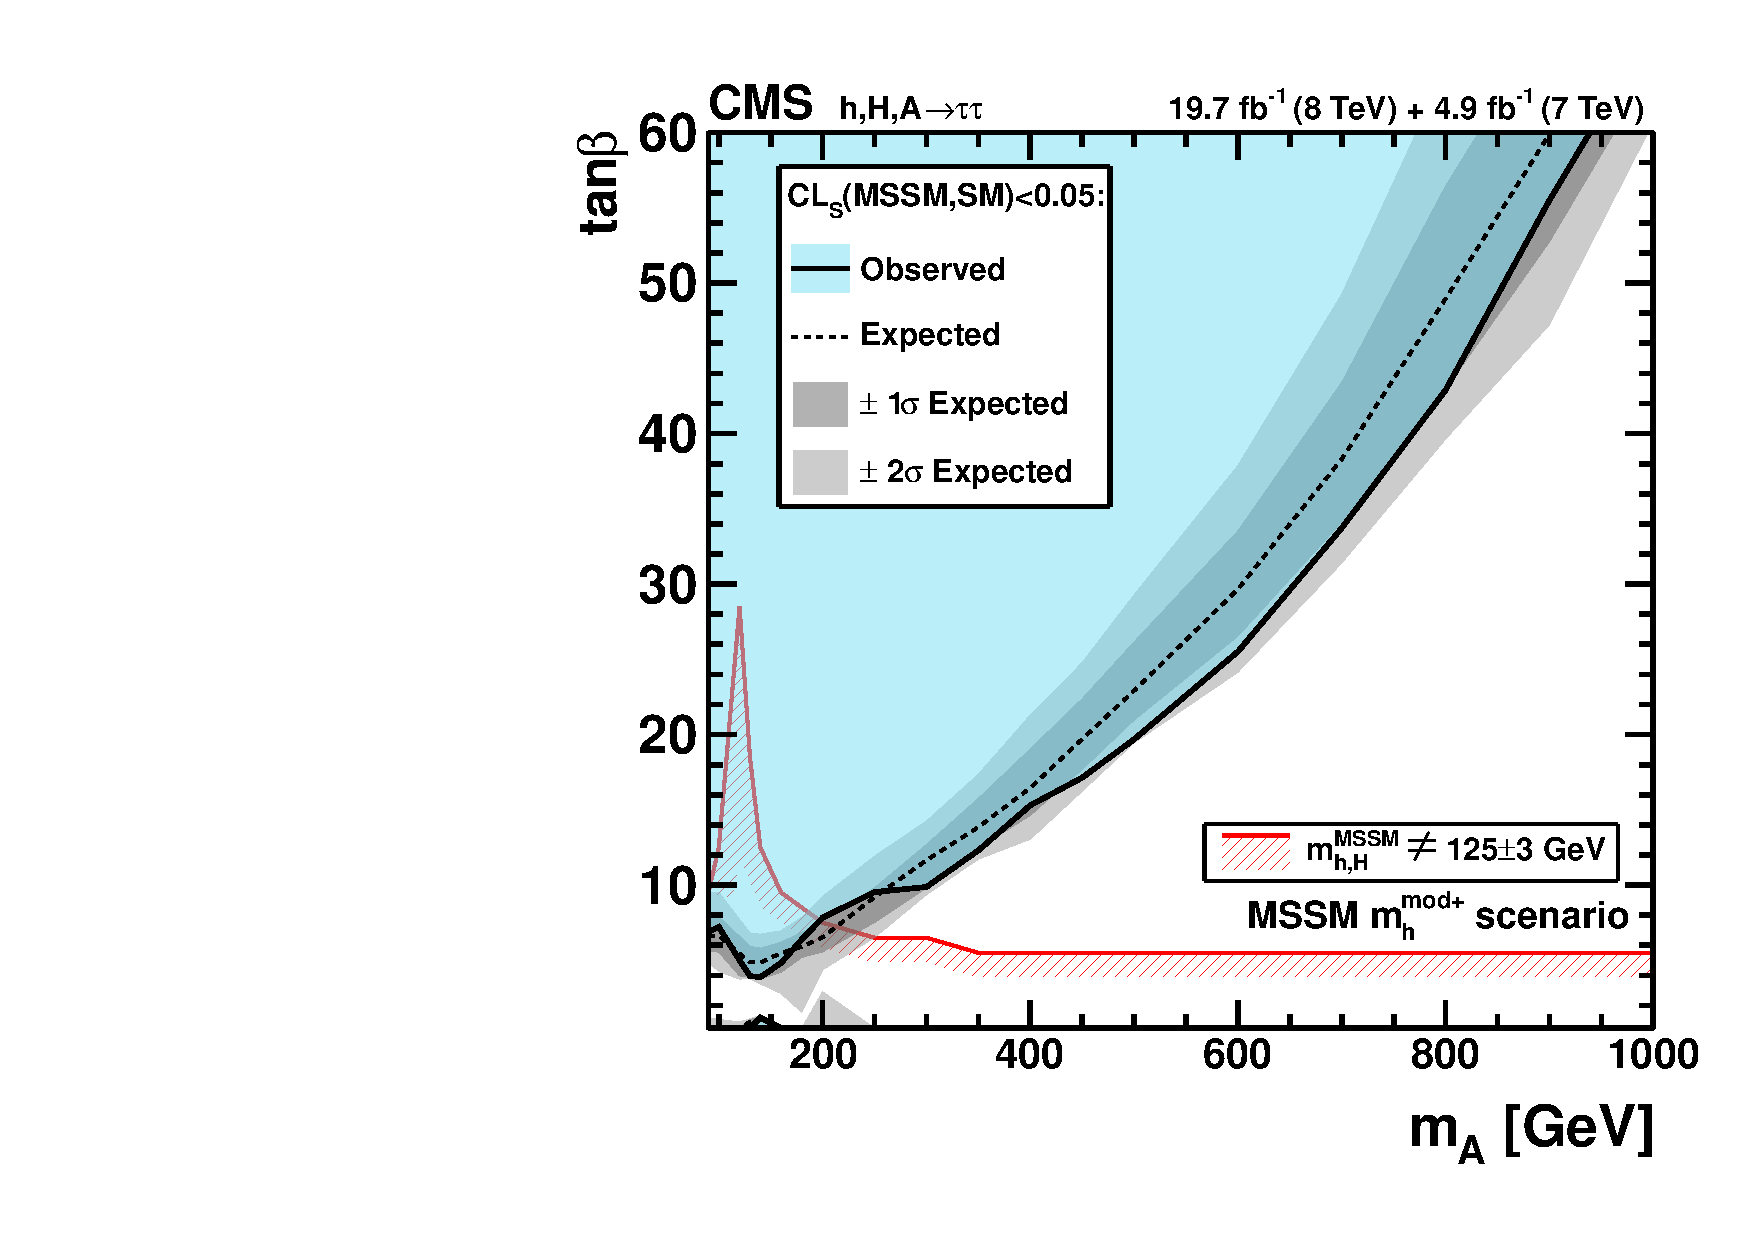
\includegraphics[width=0.5\textwidth]{plots/htt-mssm/cmbRL_mhmodp-HypoTest.pdf}}
\subfloat[]{
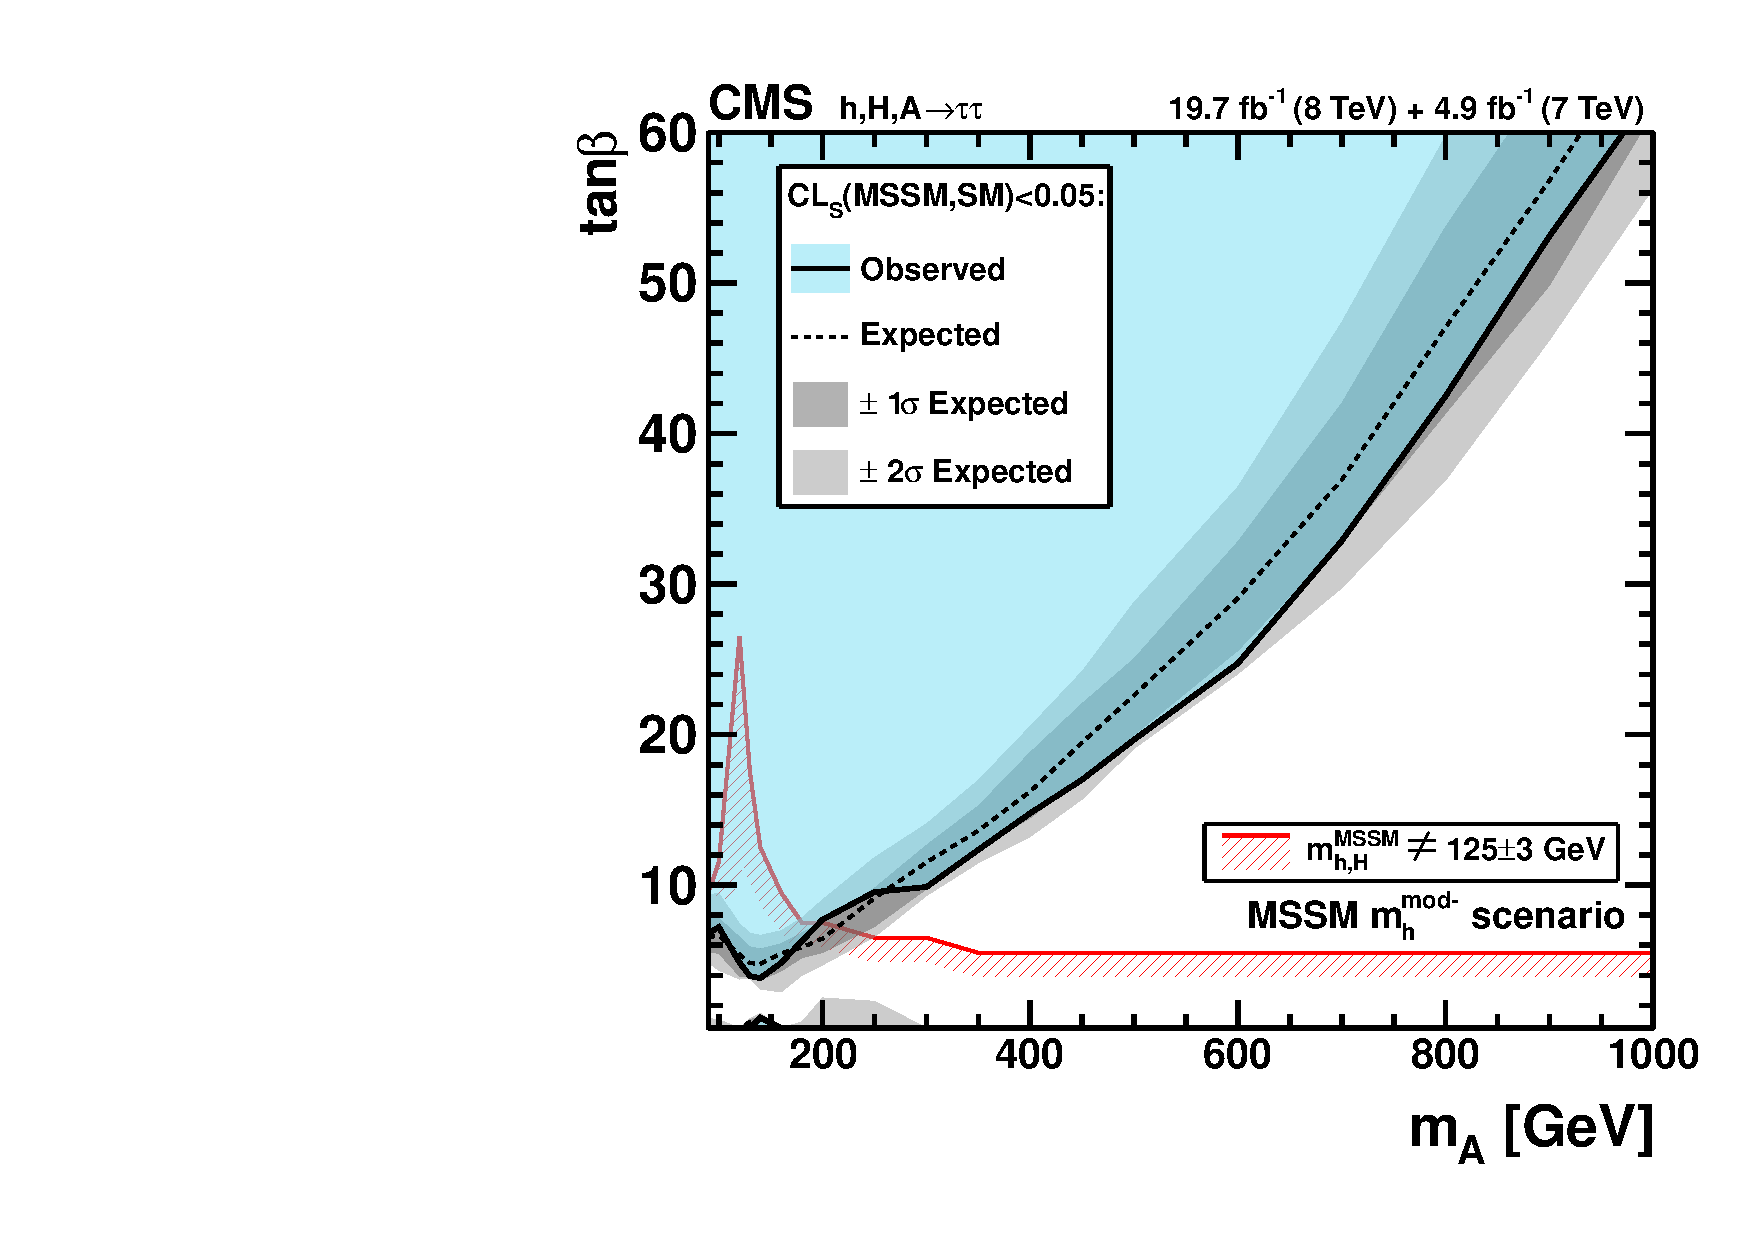
\includegraphics[width=0.5\textwidth]{plots/htt-mssm/cmbRL_mhmodm-HypoTest.pdf}}
\caption{Expected and observed limit in the $m_{\PA}-\tan\beta$ plane of the
$m_H^{\text{mod+}}$ scenario (a) and $m_H^{\text{mod-}}$ scenario (b). Hypothesis
separation testing is used to compare the \ac{MSSM} hypothesis with the \ac{SM}
hypothesis. The red area indicates the region of phase space which already
excluded by the Higgs mass constraint of $125\pm3~\GeV$ \cite{HIG-13-021}.}
\label{fig:mhmodpmhmodm}
\end{figure}

\begin{figure}[tbh]
\subfloat[]{
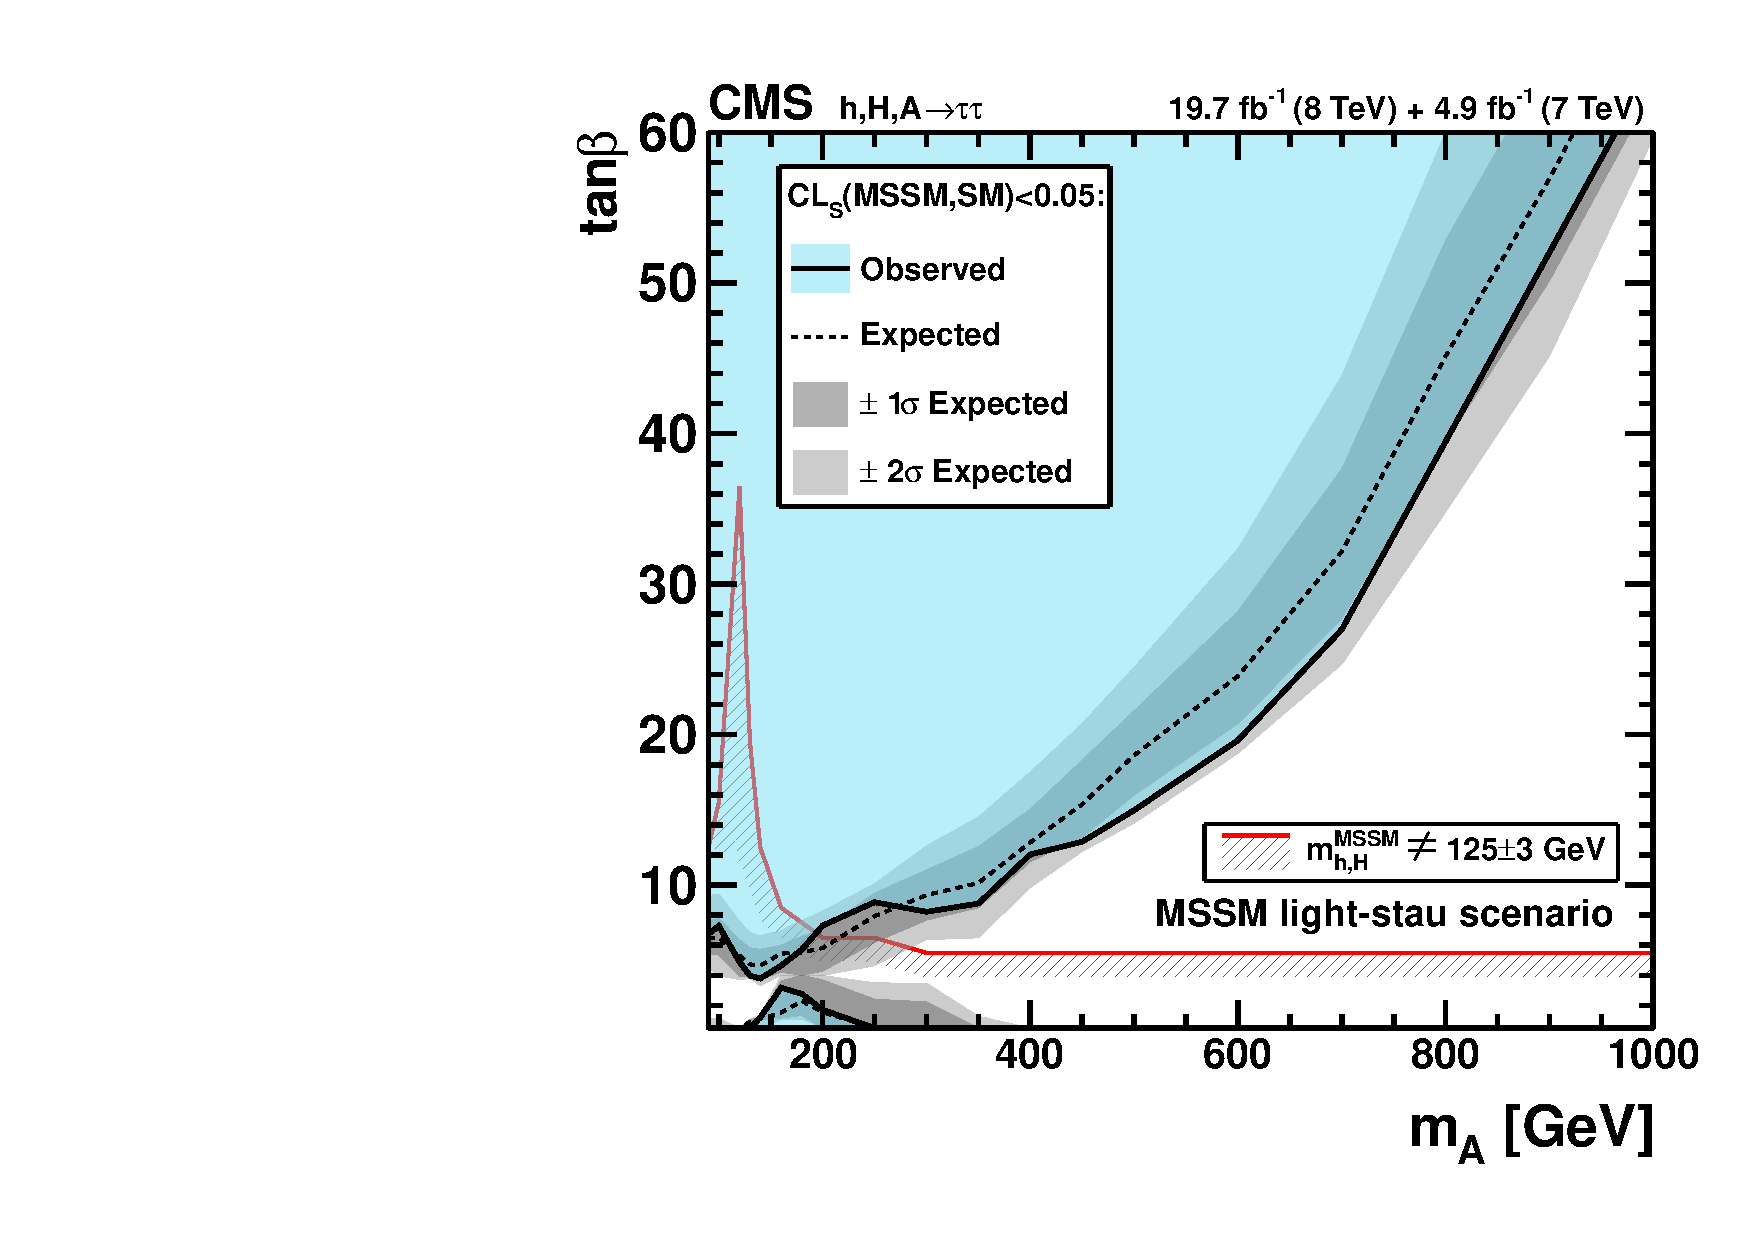
\includegraphics[width=0.5\textwidth]{plots/htt-mssm/cmbRL_lightstau1-HypoTest.pdf}}
\subfloat[]{
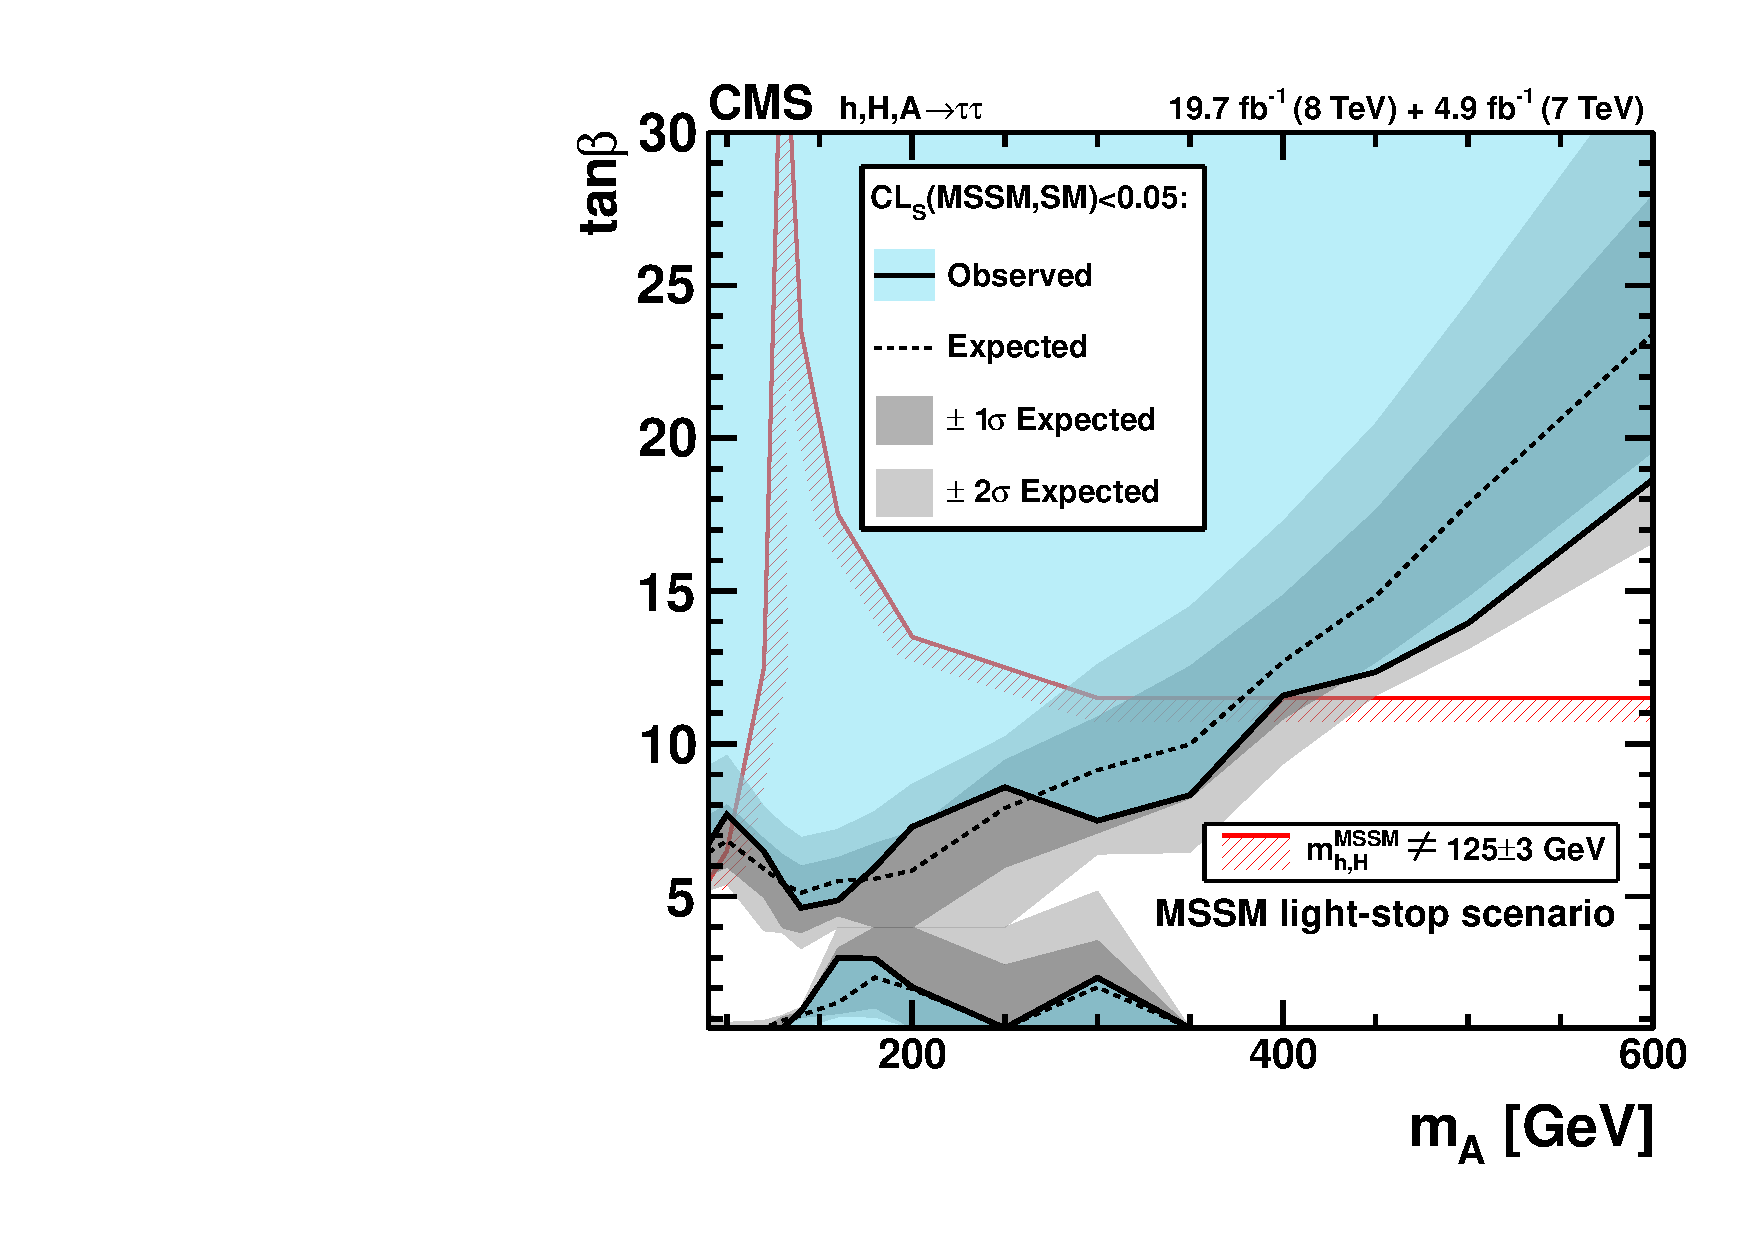
\includegraphics[width=0.5\textwidth]{plots/htt-mssm/cmbRL_lightstopmod-HypoTest.pdf}}
\caption{Expected and observed limit in the $m_{\PA}-\tan\beta$ plane of the
light-stau scenario (a) and light-stop scenario (b). Hypothesis
separation testing is used to compare the \ac{MSSM} hypothesis with the \ac{SM}
hypothesis. The red area indicates the region of phase space which already
excluded by the Higgs mass constraint of $125\pm3~\GeV$ \cite{HIG-13-021}.}
\label{fig:lightstaulightstop}
\end{figure}

\begin{figure}[tbh]
\subfloat[]{
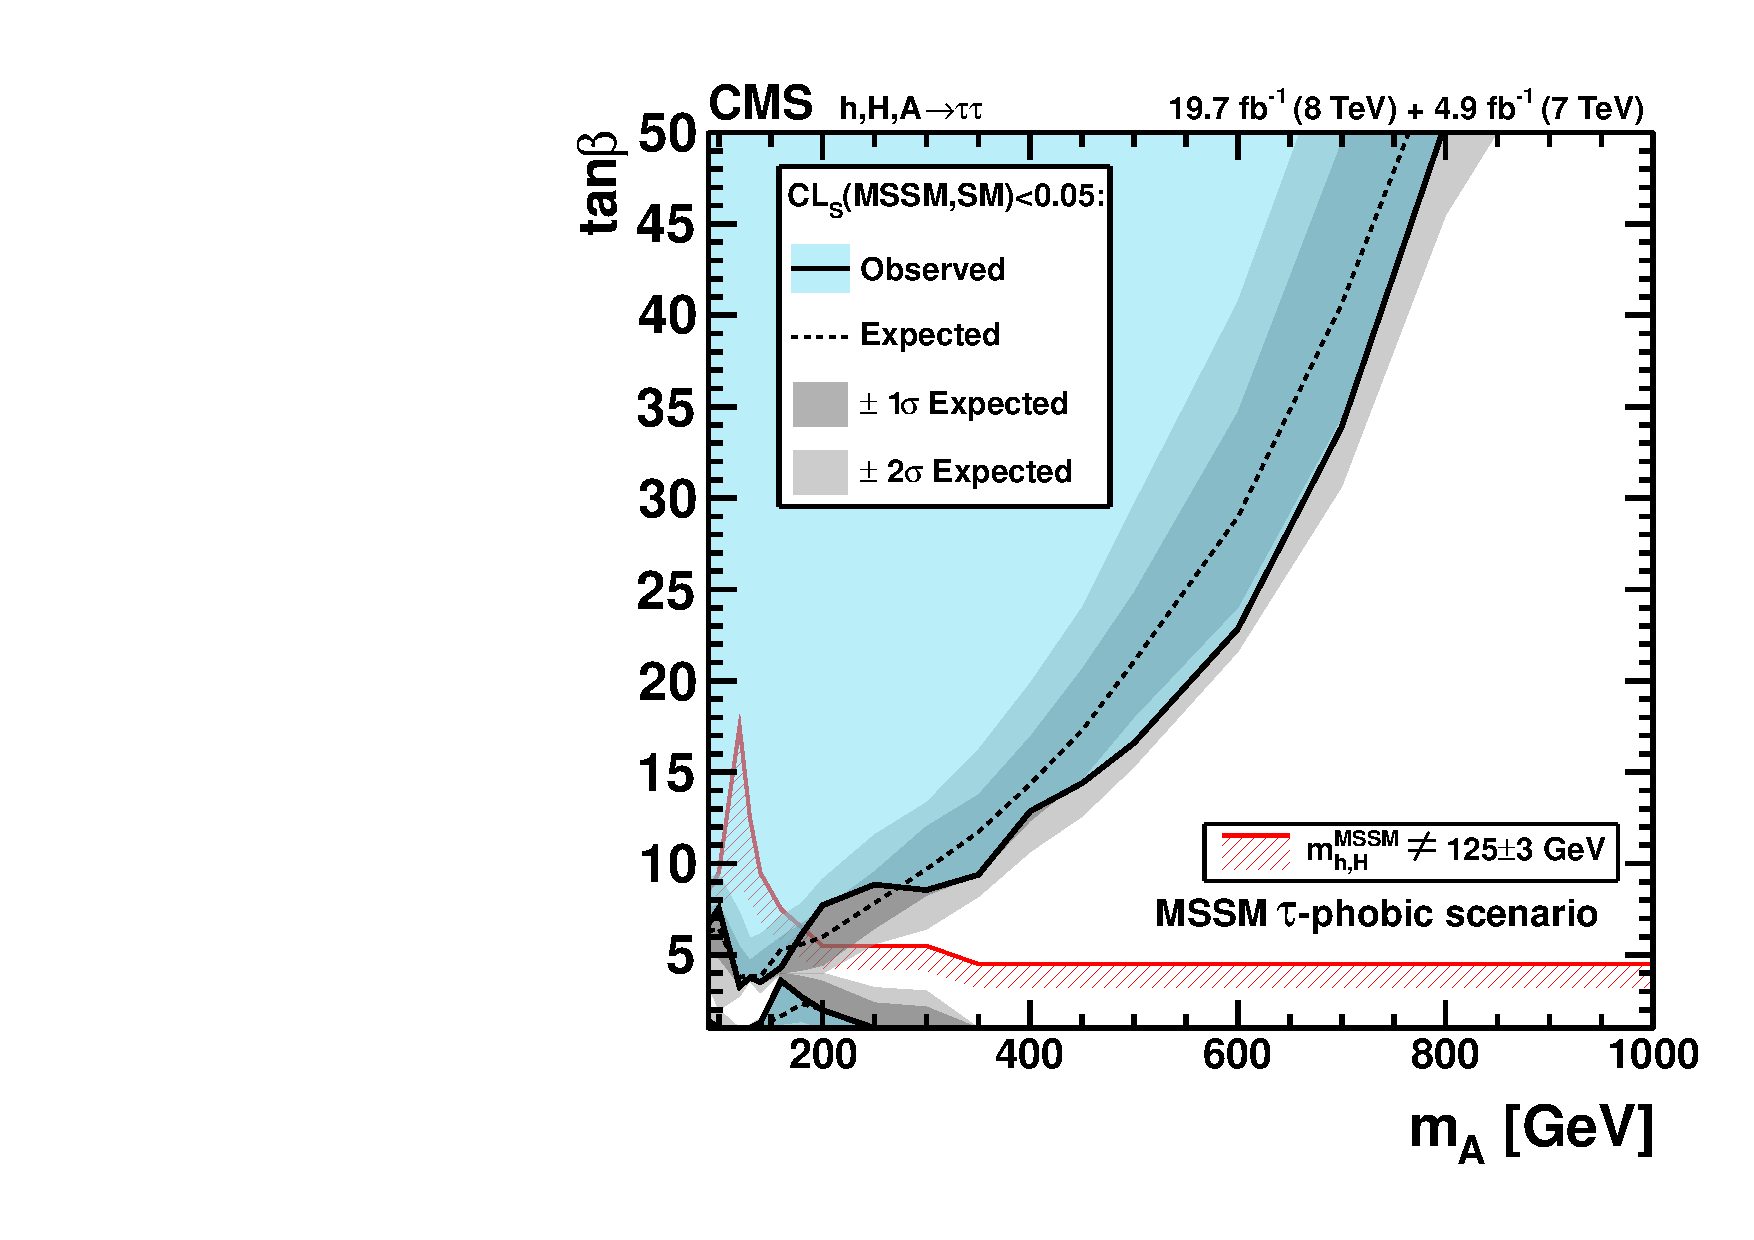
\includegraphics[width=0.5\textwidth]{plots/htt-mssm/cmbRL_tauphobic-HypoTest.pdf}}
\subfloat[]{
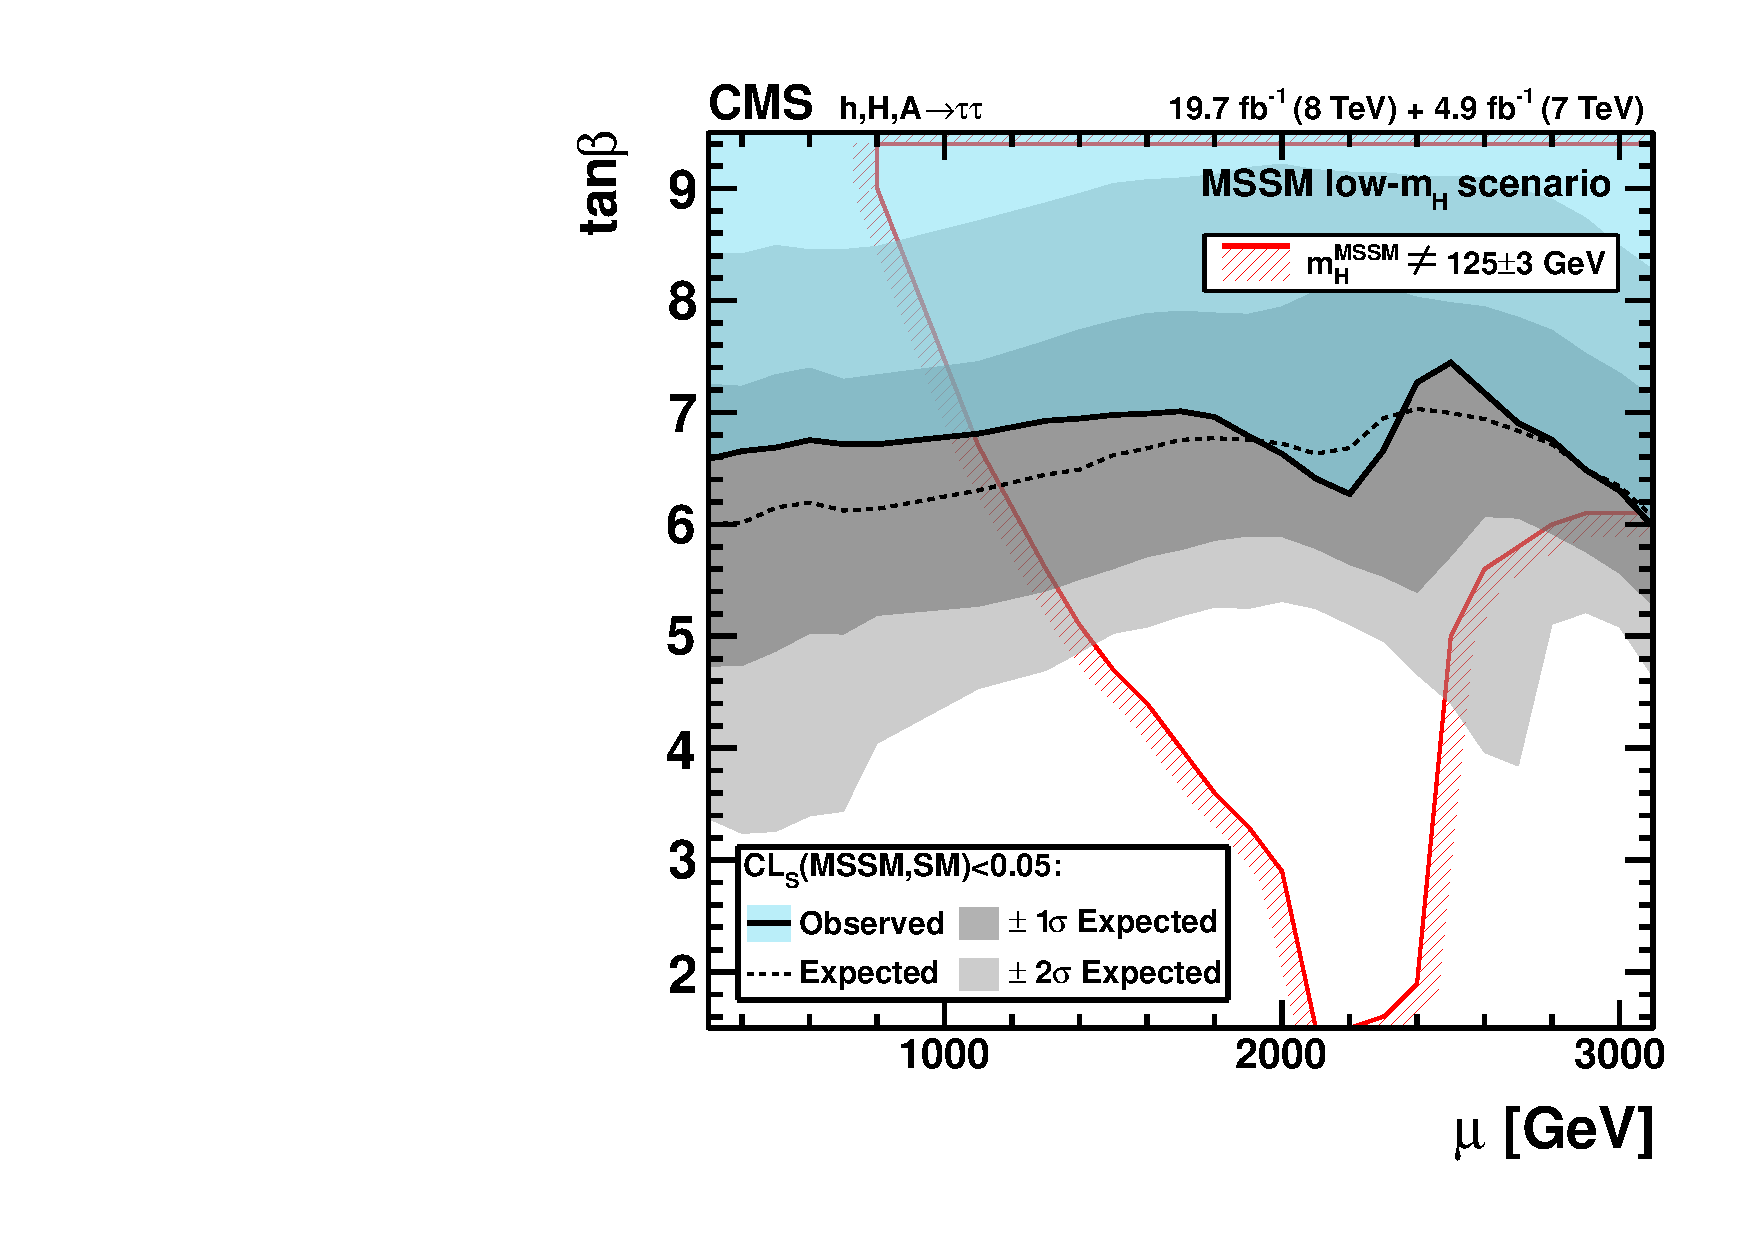
\includegraphics[width=0.5\textwidth]{plots/htt-mssm/cmbRL_lowmH-HypoTest.pdf}}
\caption{Expected and observed limit in the $m_{\PA}-\tan\beta$ plane of the
$\tau$-phobic scenario (a) and low-$m_{\PH}$ scenario (b). Hypothesis
separation testing is used to compare the \ac{MSSM} hypothesis with the \ac{SM}
hypothesis. The red area indicates the region of phase space which already
excluded by the Higgs mass constraint of $125\pm3~\GeV$ \cite{HIG-13-021}.}
\label{fig:tauphobiclowmH}
\end{figure}
